\documentclass{report}
\usepackage{arev}
\usepackage[T1]{fontenc}
\usepackage[a4paper, left=2.5cm, right= 2.5cm, top=2.5cm, bottom= 2.5cm]{geometry} %cambiar los márgenes
\usepackage{amsmath, amssymb, cancel, extarrows, amsthm }%símbolos matemáticos
\usepackage{wasysym}  %la carita triste
\usepackage{derivative}
\usepackage{physics}
\usepackage{graphicx, wrapfig}% Include figure files
\usepackage{subfig}
\usepackage{dcolumn}% Align table columns on decimal point
\usepackage{bm}% bold math
\usepackage{hyperref}% add hypertext capabilities
\usepackage{units}
\usepackage[spanish, es-tabla]{babel} %traducción al español
\usepackage{fancyhdr, ragged2e}
\setlength{\headheight}{13.07002pt}
\renewcommand{\footrulewidth}{0.4pt}
\usepackage{float}
\usepackage[symbol]{footmisc}
\usepackage{booktabs}
\usepackage{multirow}
\usepackage{multicol}
\usepackage[table,xcdraw]{xcolor}
\usepackage{xcolor, colortbl}
\usepackage{pagecolor}
\usepackage{tcolorbox}
\renewcommand{\thempfootnote}{\fnsymbol{mpfootnote}}
\newtcolorbox{mybox}{colback=gray!5!white,colframe=black!75!black}
\definecolor{cadetblue4}{rgb}{.33,.53,.55}
\definecolor{azulcrepuscular}{rgb}{.49,.62,.75}
\definecolor {atomictangerine} {rgb} {1.0, 0.6, 0.4}
\usepackage{longtable}
\usepackage{hyperref}
\hypersetup{
    colorlinks=true,
    linkcolor=black,
    filecolor=magenta,      
    urlcolor=blue,
    pdftitle={Apuntes de Geometría Diferencial \& Cálculo Tensorial},
    pdfpagemode=FullScreen,
    }

\renewcommand\familydefault{\sfdefault}
\addto\captionsspanish{
  \renewcommand{\contentsname}%
    {Índice de contenidos}%
}

\begin{document}
\newpagecolor{portada}
\begin{titlepage}
   \raggedright
       \vspace*{1cm}
       \textcolor{white}{\rule{\textwidth}{2pt}}
        \HUGE
       {\rmfamily \textbf{\textcolor{white}{Electrodinámica Clásica}}}
       
        \Large
       \vspace{0.5cm}
       {\rmfamily \textbf{\textcolor{white}{Manuel Lozano Bermúdez}}}

       \large
       \vspace{0.5 cm}
       {\rmfamily \textbf{\textcolor{white}{Curso 2023-2024, grupo C}}}
       \textcolor{white}{\rule{\textwidth}{2pt}}
        \vspace{1.5 cm}
       \begin{figure}[h]
           \centering
           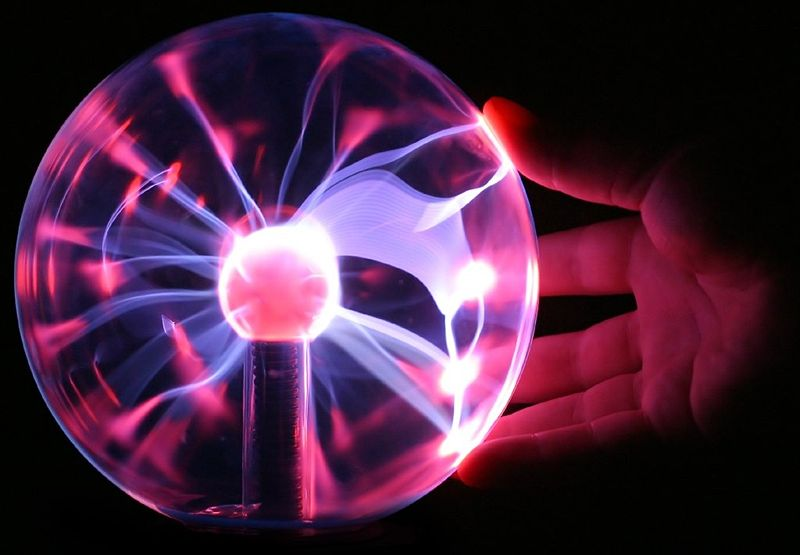
\includegraphics[scale=.4]{FOTOS/portada.jpg}
           \label{fig:portada}
       \end{figure}

        \vspace*{\fill}
        
         \Large
         {\rmfamily \textcolor{white}{Comenzado el: 6 de septiembre de 2023}\\}
         {\rmfamily \textcolor{white}{Terminado el: 25 de septiembre de 2023 (SIN ACABAR)}}


\end{titlepage}
\restorepagecolor

\pagestyle{fancy}
\fancyhead[R]{}
\fancyfoot[L]{Manuel Lozano B.}
\fancyfoot[R]{GD$\&$CT}

\section*{Agradecimientos}

A Marcos, por revisar los apuntes, limpiarlos de erratas y por obligarme a mantener frescos mis conocimientos de la  asignatura. 

\tableofcontents

\part{Teoría}

\chapter[DFT]{Density Functional Theory}
\section[ITRO. DFT (SHOLL)]{Introducción a la teoría DFT [\emph{Sholl}]}

La teoría DFT o \emph{Teoría de Densidad del Funcional} está basada en dos bucles auto consistentes.
\begin{enumerate}
    \item En el primer bucle, se busca la \textbf{densidad electrónica más estable} para determinar la configuración atómica.
    \item En el siguiente bucle, se busca la configuración atómica que \textbf{minimice la energía total del sistema}.
\end{enumerate}
Pueden llegar a ocurrir diferentes cosas: 
\begin{itemize}
    \item Se llegan a diferentes configuraciones finales del sistema con la misma energía. La más estable de ellas será la que aceptemos.
    \item Puede ocurrir que una configuración atómica dada tenga diferentes mínimos de energía estables. En esos casos, aparecen \textbf{dominios} en el material (que es el origen, por ejemplo, de los dominios magnéticos de un ferromagnético).
\end{itemize}

La característica fundamental de esta teoría es que se tratará a los electrones como \textbf{densidades}, $n(\B{r})$ o $\rho(\B{r})$ (dependiendo del libro). Estas densidades se definen\footnote{Una definición más acertada tendría en cuenta un factor 2 multiplicando debido al \emph{espín}: $$n(\B{r}) = \textcolor{red}{2}\sum_i \psi_i(\B{r})^* \psi_i(\B{r})$$} en términos de las funciones de onda de electrones independientes, $\{\psi_i\}$: 
\begin{equation}
    \rho(\B{r})\equiv n(\B{r}):=\sum_i |\psi_i(\B{r})|^2 = \sum_i \psi_i(\B{r})^* \psi_i(\B{r})
\end{equation}
Esta teoría esta basada en dos teoremas fundamentales de \emph{Hohenberg} y \emph{Kohn}. El primero enuncia que la densidad electrónica determina \emph{completamente} la energía del estado fundamental. Dicho de otra forma, \textbf{la energía del estado fundamental es un funcional dependiente únicamente de la densdiad electrónica}, es decir, $E\equiv E[n(\B{r})]$. Este es un resultado fundamental ya que permite reducir considerablemente la dimensionalidad del problema, pasando de considerar $N$ átomos en nuestra red a centrarnos únicamente en nuestra densidad electrónica, de tres dimensiones espaciales. No obstante, con este teorema únicamente no tenemos ninguna información sobre la forma de esa densidad $n(\B{r})$, por ello la necesidad del segundo teorema. \\

En el segundo teorema, se establece que \textbf{la densidad electrónica real} que representa a nuestro sistema es aquella que \textbf{minimiza la energía} (del estado fundamental). Esto implica que si conociésemos la relación funcional real de la densidad electrónica, podríamos variarla hasta encontrar la que minimiza la energía.\\

El siguiente paso es aproximar. Una aproximación útil (y en la cual permaneceremos a lo largo del proyecto) es en la de \textbf{electrones libres}, es decir, sin interacciones entre ellos. De esta manera, se puede llegar a un funcional de la energía aproximado dado por
\begin{equation} \label{1.1}
    E[\{ \psi_i \}] = E_\text{conocido}[\{ \psi_i \}] + E_\text{XC}[\{ \psi_i \}] \ .
\end{equation}
\begin{itemize}
    \item El término $E_\text{conocido}[\{ \psi_i \}]$ corresponde a los términos que conocemos analíticamente, que son las energías cinéticas de los electrones (KE), interacciones electrón-núcleo, electrón-electrón y núcleo-núcleo de tipo coulombianas (EN, EE y NN, respectivamente).
    \begin{equation}
        E_\text{conocida}[\{ \psi_i \}]=\underbrace{-\frac{\hbar^2}{2m} \sum\nolimits_i \int \psi_i^* \laplacian \psi_i \D[3]{r}}_{\text{KE}} + \underbrace{\int V(\B{r})n(\B{r}) \D[3]{r}}_{\text{EN}} + \underbrace{\frac{e^2}{2}\iint \frac{n(\B{r})n(\B{r'})}{|\B{r}-\B{r'}|} \D[3,3]{r,r'}}_{\text{EE}} + E_\text{NN}
    \end{equation}

    \item El término $E_\text{XC}[\{ \psi_i \}]$ corresponde al funcional de correlación-canje, que incluye el resto de efectos mecano-cuánticos no tenidos en cuenta. De momento no tenemos nada de información sobre él.
\end{itemize}

Suponiendo que conozcamos la forma funcional del término de canje-correlación, necesitamos una manera de encontrar las funciones de onda $\{\psi_i\}$ de manera sencilla. Esto se consigue resolviendo las \emph{ecuaciones de Kohn-Sham}, que reducen esta tarea laboriosa a resolver la ecuación de Schrödinger para un solo electrón.
\begin{equation}
    \left [-\frac{\hbar^2}{2m}\laplacian +V(\B{r}) + V_H(\B{r}) + V_\text{XC}(\B{r}) \right ]\psi_i(\B{r}) = \varepsilon_i\psi_i(\B{r})
\end{equation}
\begin{itemize}
    \item El potencial $V(\B{r})$ corresponde a la interacción entre un electrón y el conjunto de los núcleos atómicos.
    \item El potencial $V_H(\B{r})$ se conoce como \textbf{potencial de Hartree}, definido como:
    $$
     V_H(\B{r})=e^2\int \frac{n(\B{r'})}{|\B{r}-\B{r'}|} \D[3]{r'} \ .
    $$
    Describe la interacción de repulsión coulombiana entre el electrón considerado y el conjunto de electrones dentro de la densidad electrónica. Como el electrón considerado también pertenece a $n(\B{r})$, este potencial describe una auto-repulsión hacia el electrón. Para corregir esa auto-repulsión, se añade un término correspondiente dentro de $V_\text{XC}$.

    \item El potencial $V_\text{XC}$ describe las contribuciones de correlación-canje {\scriptsize (lol gracias sara)}. Puede expresarse formalmente como una  \emph{derivada funcional} \footnote{Más información de derivadas funcionales: \url{https://es.wikipedia.org/wiki/Derivada_funcional} .}:
    $$
    V_\text{XC}(\B{r}) = \fdv{E_\text{XC}}{n(\B{r})}
    $$
\end{itemize}

Para calcular la función de onda del electrón necesitamos la densidad electrónica, pero para calcular la densidad electrónica necesitamos la función de onda del electrón. El cálculo es circular, pero una manera de solventarlo es implementar un método iterativo, que es en donde entra en juego el primer bucle auto consistente que mencionábamos al principio.

\newpage

\section[INTRO. DFT (FOR BEGINNERS)]{Introducción a la DFT [\emph{DFT for beginners}]}
De la misma manera, partimos de la \emph{ecuación de Schrödinger}
\begin{equation}
    \hat{H}_S \Phi\left ( \{ \B{r}_i \} , \{ \B{R}_\alpha  \} \right ) = E_\text{TOT} \Phi \left ( \{ \B{r}_i \} , \{ \B{R}_\alpha  \} \right )
\end{equation}
donde $\{ \B{r}_i\}$ y $\{ \B{R}_\alpha\}$ son las coordenadas de los electrones y de los iones, respectivamente. El hamiltoniano es:
\begin{equation}
    \hat{H}_S = \sum _\alpha \frac{P_\alpha ^2}{2M_\alpha } + \sum _i \frac{p_i^2}{2m_i} + \frac{1}{2} \sum_{i\neq j} \frac{1}{|\B{r}_i - \B{r}_j |} - \sum _{i,\alpha } \frac{Z_\alpha }{|\B{r}_i - \B{R}_\alpha |} + \frac{1}{2} \sum_{\alpha \neq \beta } \frac{Z_\alpha Z_\beta }{|\B{R}_\alpha - \B{R}_\beta |}
\end{equation}
\subsection{1ª aproximación: Born-Oppenheimer (electrones independientes)}
Separamos el movimiento electrónico del iónico.
\begin{equation}
    \left ( \hat{H}_S - \sum_\alpha \frac{P_\alpha ^2}{2M_\alpha } \right ) \Psi_{\{ \B{R}_\alpha  \} } (\{ \B{r}_i \}) = E_\text{fund}(\{ \B{R}_\alpha  \}) \Psi {\{ \B{R}_\alpha  \} } (\{ \B{r}_i \})
\end{equation}
La energía total se convierte en
\begin{equation}
    E_\text{TOT} = \sum_\alpha \frac{P_\alpha ^2}{2M_\alpha } + E_\text{fund} (\{ \B{R}_\alpha  \})\ .
\end{equation}
Las fuerzas que actúan sobre los iones son :
\begin{equation}
    \B{F}_\beta = -\pdv{E_\text{fund}}{\B{R}_\beta } \ (\{ \B{R}_\alpha  \})
\end{equation}
\subsection{2ª aproximación: Hohenberg-Kohn}
Los electrones pasan a representarse mediante densidades electrónicas.
$$
e^- \longrightarrow \rho(\B{r}) = N_e \int \left | \Psi \left (\{ \B{r}_i \}_{i=1}^N  \right ) \right |^2 \D{\B{r}_1}\ldots \D{\B{r}_N}
$$
\subsection{3ª aproximación: [2º Teorema de Hohenberg-Kohn]}
Los potenciales de la forma $v(\B{r})=\sum_\alpha -Z_\alpha /|\B{r}-\B{R}_\alpha |$ presentan funcionales \textbf{únicos} de densidades electrónicas:
\begin{equation}
    E\equiv E[\rho(\B{r})]
\end{equation}
Esto lleva a definir la energía fundamental como:
\begin{equation}
    E_\text{fund} = E[\rho_\text{fund}] + \frac{1}{2} \sum _{\alpha \neq \beta } \frac{Z_\alpha Z_\beta }{|\B{R}_\alpha - \B{R}_\beta |}
\end{equation}
\subsection{4ª aproximación: Ecuaciones de Kohn-Sham}
El problema de resolver N ecuación de Schrödinger puede simplificarse a resolver una única ecuación de un electrón independiente:
\begin{equation}
    E[\rho] = \int v(\B{r}) \rho (\B{r}) \D{\B{r}} + E_{ee}[\rho] + T_S [\rho] + E_{XC} [\rho]
\end{equation}
\begin{itemize}
    \item $E_{ee}$ es la energía de interacción (coulombiana) electrón-electrón:
    $$
    E_{ee} := \frac{1}{2} \iint \frac{\rho(\B{r}) \rho(\B{r}')}{|\B{r} - \B{r}'|} \D{\B{r},\B{r}'}
    $$

    \item $T_S[\rho] $ es la energía cinética de electrones no interactuantes entre sí, para $\rho(\B{r}) = \sum_{n=1} ^{N_e} |\psi_n(\B{r})|^2$ . 
    \begin{equation*}
        \begin{split}
                \left [ -\frac{1}{2}\laplacian + V(\B{r}) \right ] \psi_n (\B{r}) &= \varepsilon_n \psi_n (\B{r})\\
                                                                        T_S[\rho] &= \sum_{n=1} ^{N_e} \varepsilon_n - \int V(\B{r}) \rho (\B{r}) \D{\B{r}}                                \\
                                                                         V(\B{r}) &= v(\B{r}) + \int \frac{\rho(\B{r}')}{|\B{r}-\B{r}'|} \D{\B{r}'} + \fdv{E_{XC}}{\rho }\\
                                                                                  &= v(\B{r}) + V_H(\B{r}) + V_{XC}(\B{r})
        \end{split}
    \end{equation*}
\end{itemize}
Observamos que para obtener los orbitales electrónicos, necesitamos la densidad electrónica; pero para obtener la densidad electrónica, necesitamos los orbitales electrónicos. Para encontrar ambos, creamos un bucle auto consistente y la densidad de estados en cada iteración se convierte en una combinación de la de entrada y salida del bucle.
\begin{figure}[h!]
    \centering
    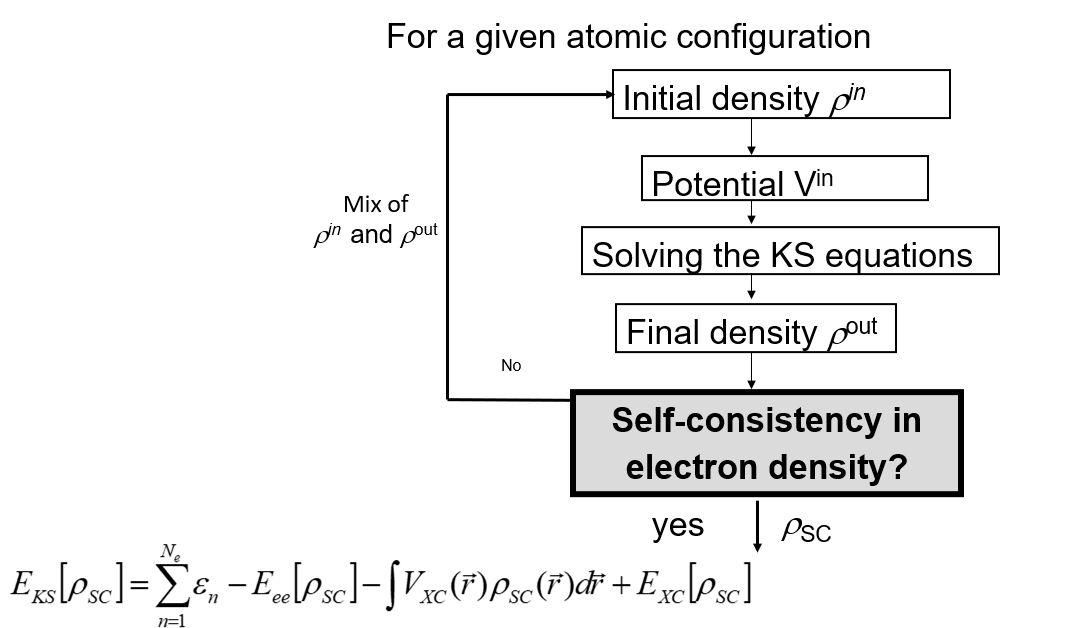
\includegraphics[scale=.4]{FIGURAS/bucle dft.png}
    \label{fig:bucle}
\end{figure}

\subsection{Otras aproximaciones}
\begin{itemize}
    \item \textbf{Aproximación de pseudo-potencial: } Bajo esta aproximación, los electrones de capas más internas se integran con el núcleo y se toman en cuenta únicamente las contribuciones a enlaces de los electrones de la capa de valencia. Esto reduce el número de variables a tener en cuenta en el cálculo.

    \item \textbf{Correlación y canje: }Para modelar el término de correlación y canje se pueden llevar a cabo diferentes tipos de aproximaciones, siendo la más sencilla la LDA (\emph{Local Density Approximation}). Según el modelo LDA, la energía en un punto $r$ corresponde a la energía de un gas electrónico homogéneo con la misma densidad electrónica en ese punto.
    \begin{equation*}
        \begin{split}
            E_{XC}{}^{(LDA)}[\rho ]&=\int \varepsilon_{XC} (\rho) \rho(\B{r}) \D{r} \implies V_{XC}{}^{(LDA)}=\pdv{[\rho(\B{r})\varepsilon_{XC}(\rho)]}{\rho(\B{r})}\\
            \varepsilon_{XC} &= \varepsilon_{XC}{}^\text{hom}[\rho]
        \end{split}
    \end{equation*}

    \item \textbf{Aproximación ión-ión: enfoque de Ewald.} Para lidiar con la suma de infinitos términos en el término de interacción ión-ión, se introduce un parámetro $\eta$ para hacer converger rápidamente la suma.
\end{itemize}

\chapter{Superficies. Primera forma fundamental y cálculo tensorial}

\section{Concepto de superficie}
\large 

Un subconjunto $S\subseteq \mathbb{R}^3$ es una \emph{superficie regular} de $\mathbb{R}^3$ si para cada punto $P\in S$ existe un conjunto abierto de $\mathbb{R}^2$, $U\subseteq \mathbb{R}^2$, un conjunto abierto $V\subseteq \mathbb{R}^3$ y una aplicación:
\begin{align*}
    \mathbf{x}:U\subseteq \mathbb{R}^2 &\longrightarrow V \cap S\\
    (u,v)& \longmapsto \mathbf{x}(u,v)=(x(u,v),y(u,v),z(u,v))
\end{align*}
tal que:
\begin{enumerate}
    \item[(i)] $\mathbf{x}:U\rightarrow V\cap S$ es de clase $C^\infty (U)$, (es decir, $x((u,v), y(u,v), z(u,v))$ son funciones de clase $C^\infty $ en su dominio).

    \item[(ii)] $\mathbf{x}:U\rightarrow V\cap S$ es un \emph{homomorfismo}, es decir, es \emph{biyectiva} (uno a uno), y su aplicación inversa es continua (esta condición evita que la superficie tenga auto intersecciones). 

    \item[(iii)] $\mathbf{x}:U\rightarrow V\cap S$ es \emph{regular}, es decir, su imagen es bidimensional, si la matriz jacobiana de derivadas es de rango 2 en $U$.
    $$
    J(u,v)=D\mathbf{x}=\left ( 
    \begin{array}{cc}
         \pdv{x(u,v)}{u}&\pdv{x(u,v)}{v}  \\\\
         \pdv{y(u,v)}{u}&\pdv{y(u,v)}{v}  \\\\
         \pdv{z(u,v)}{u}&\pdv{z(u,v)}{v}
    \end{array}
    \right )\longrightarrow rg(J)=2 \ , \ \forall (u,v)\in \mathbb{R}^2
    $$

    Esta condición evita que tengamos casos degenerados, como puntos o rectas (por ejemplo: $\mathbf{x}(u,v)=(u+v,u+v,u+v)$, que es en realidad una recta $\mathbf{x}(t)=(t,t,t)$).
\end{enumerate}

\paragraph{Notación:} Al par $(U,\mathbf{x}(u,v))$ se le denomina \emph{carta} (o entorno) local de la superficie $S$ (típicamente en torno a un punto $P \in S$). La carta proporciona un sistema de coordenadas a través de una parametrización local de la superficie.
\newpage
\begin{wrapfigure}{l}{0.43\textwidth}
    \centering
    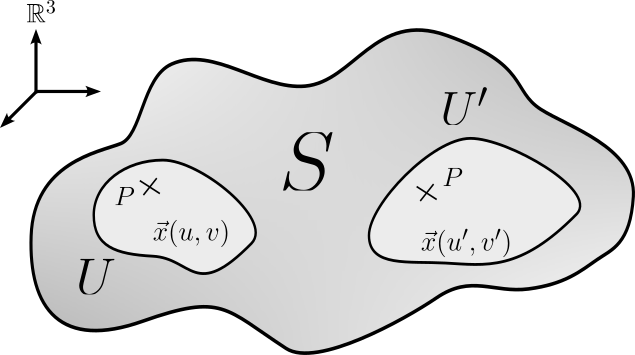
\includegraphics[scale=.4]{FOTOS/carta.png}
\end{wrapfigure}

La suma de todas las cartas que permiten cubrir completamente una superficie se conoce como \emph{atlas}. \\

Una superficie como $\mathbb{R}^2$ puede cubrirse mediante un atlas con una única carta (se conoce como superficie trivial). Si esta no es trivial, puede que hagan falta más de una carta para cubrir la superficie entera, como en el caso de la esfera o del cono, como se verá en el siguiente ejemplo.\\

\begin{mybox}
    \underline{Ejemplo A:} \\
        (i) El plano $XY$ puede cubrirse con una única carta:
        
        \begin{wrapfigure}{r}{0.25\textwidth}
            \centering
            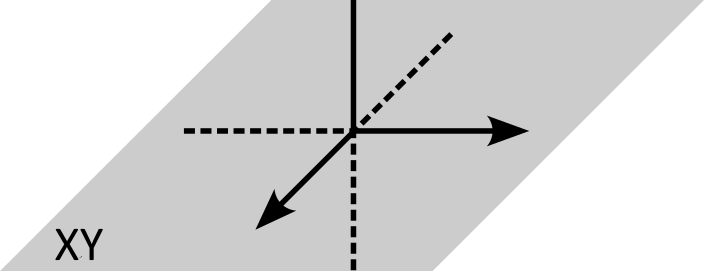
\includegraphics[scale=.2]{FOTOS/ejemplo2_A.png}
            \caption*{(i)}
        \end{wrapfigure}
        
        \begin{gather*}
        \mathbf{x}(u,v)=(u,v,0) \ , \text{con }u,v \in \mathbb{R}\\
        J(u,v)=\left ( \begin{array}{cc}
             1&0  \\
             0&1  \\
             0&0
        \end{array} \right ) \longrightarrow rg(J)=2 \ ; \ \forall u,v 
        \end{gather*}
        Lo mismo ocurre con las gráficas de las funciones de dos variables (representación en la carta de Monge):
        \begin{align*}
            f:U\subseteq \mathbb{R}^2 &\longrightarrow\mathbb{R}^3\\
                                 (x,y)&\longmapsto f(x,y)  \implies \mathbf{x}(u,v)=(u,v,f(u,v)) \text{ que tiene } rg(J)=2
        \end{align*}
            \begin{wrapfigure}{l}{0.2\textwidth}
             \centering
             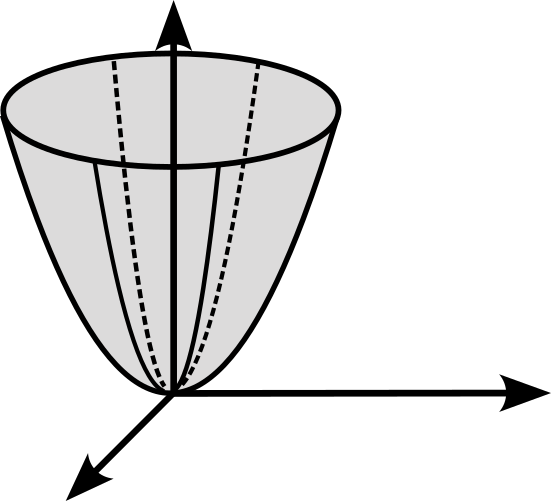
\includegraphics[scale=.18]{FOTOS/ejemplo2_A_2.png}
             \caption*{(ii)}
             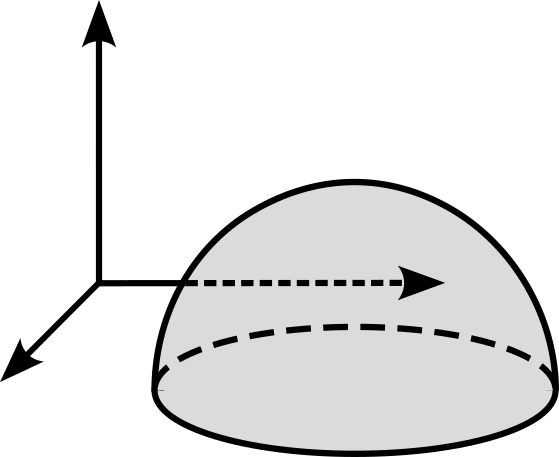
\includegraphics[scale=.18]{FOTOS/ejemplo2_A_4.png}
             \caption*{(iv)}
         \end{wrapfigure}
         (ii) El paraboloide de revolución $z=x^2+y^2$ se puede cubrir también con una carta:
        $$
        \mathbf{x}(u,v)=(u,v,u^2+v^2) \ , \ \text{con }u,v\in \mathbb{R} 
        $$
         (iii) El paraboloide hiperbólico $x=x^2-y^2$ se puede cubrir con la carta 
         $$\mathbf{x}(u,v)=(u,v,u^2-v^2)$$
         (iv) La semiesfera (\emph{hemisferio}) $z=\sqrt{1-x^2-y^2}$ (tomado de la esfera-- que \textbf{no} es una función--: $x^2+y^2+z^2=1$). Esta superficie \textbf{no} es regular a no ser que eliminemos de su dominio el ecuador (ya que para que sea regular, sus derivadas tienen que estar bien definidas, algo que no pasa cuando $z=0$). En este caso, la carta es: 
         $$
         \mathbf{x}(u,v)=\left (u,v,\sqrt{1-u^2-v^2}\right ) \ , \ U=\{ (u,v)\in \mathbb{R}^2 :u^2+v^2<1 \}
         $$
         
         (v) El cilindro $S=\{ (x,y,z)\in \mathbb{R}^3:x^2+y^2=1 \}$ (en coordenadas cilíndricas):
         $$
         \mathbf{x}(u,v)=(\cos u , \sin u , v) \ , \ u \in (0,2\pi),v\in \mathbb{R}
         $$
\end{mybox}
\begin{mybox}
         Para cubrir el cilindro, es decir, el atlas del cilindro, hacen falta \emph{dos} cartas (la razón es que el cilindro no se parece a $\mathbb{R}^2$ al tener una recta en la que está multievaluada. Esto implica que hagan falta operaciones para convertirlo en algo semejante a $\mathbb{R}^2$). \emph{No obstante, si se elimina una recta del cilíndro sí que puede cubrirse con una carta.}\\
         %AÑADIR DIBUJO

         (vi) La esfera $x^2+y^2+z^2=1$ implica que se necesitan seis cartas para cubrir el atlas, pero si usamos coordenadas esféricas necesitamos dos.
         $$
         \left \{ 
         \begin{array}{ccc}
             x &=& \pm \sqrt{1-y^2-z^2} \\
             y &=& \pm \sqrt{1-x^2-z^2} \\
             z &=& \pm \sqrt{1-x^2-y^2} \\
         \end{array}
         \right . \Longrightarrow\left \{
         \begin{array}{c}
              \mathbf{x}(u,v)=(\sin u \cos v, \sin u \sin v , \cos u)  \\
              U=\left \{ (u,v)\in \mathbb{R}^2:
              \begin{array}{c}
                   0<v<2\pi   \\
                   0<u<\pi 
              \end{array}
              \right \}
         \end{array} \right .
         $$

         %AÑADIRDIBUJOOOOO

         (vii) Cono: $S=\left \{ (x,y,z)\in \mathbb{R}^3: z=\sqrt{x^2+y^2} \right \}$. Esta superficie tiene un problema de derivabilidad en el origen de coordenadas (pico), por lo que \textbf{no} es regular en ese punto. Para construir una carta de la superficie podemos trabajar en coordenadas cilíndricas. En este caso necesita dos cartas \footnote[1]{Como con el cilindro, puede cubrirse con una carta si se elimina una recta.}:
         $$
         \mathbf{x}(u,v)=(u\cos v, u\sin v , v), \qquad 0<u<\infty , 0<v<2\pi 
         $$

         (viii) Helicoide (escalera de caracol): $\mathbf{x}(u,v)=(u \cos v, u\sin v, v$, con $0<u<\infty $ y $v\in \mathbb{R}$.

         %DIBUJOOOO
\end{mybox}


\section{Curvas en una superficie}
%DIBUJOOO

Sea una superficie regular $S$ y una carta local $(U,\mathbf{x}(u,v))$ de dicha superficie; y sea la aplicación $\mathbf{\sigma}$,
\begin{align*}
    \mathbf{\sigma}:I\in \mathbb{R}&\longrightarrow U\subseteq \mathbb{R}^2\\
    t&\longmapsto \mathbf{\sigma}(t)=(u(t),v(t)),
\end{align*}
suficientemente suave, es decir, de clase $C^r$ con $r\ge 1$ en el intervalo $I$. La aplicación $\mathbf{\sigma}(t)$ representa una curva dentro de la superficie S, en concreto dentro de $U$. 
$$
\mathbf{x}(u(t),v(t))=(x(u(t),v(t)),y(u(t),v(t)),z(u(t),v(t)))
$$
\subsection{Curvas coordenadas y coordenadas curvilíneas}
Dado un punto $P(u_0,v_0)$ hay dos curvas importantes que pasan por él, que son las curvas \emph{paralelas a los ejes} $u,v$, y se conocen como \emph{curvas coordenadas}.\\

%AÑADIR DIBUJOOO

Las curvas coordenadas generan una malla que recubre completamente la superficie. Por otro lado, estas coordenadas $u,v$ son lo que se conoce como \emph{coordenadas curvilíneas} sobre la superficie $S$, asociadas a una cierta carta local $(U,\mathbf{x}(u,v))$.

\subsection{Vectores tangentes a la superficie $S$ y espacio o plano tangente}
En cada punto de $S$ hay dos valores únicos de $u$ y $v$, en el cual podemos definir dos vectores tangentes a la superficie, mediante las derivadas parciales direccionales, a lo largo de la dirección $\mathbf{x}_u$ (y lo mismo para la dirección $v$).
$$
\mathbf{x}_u=\pdv{\mathbf{x}}{u}=\left ( \pdv{}{u}x(u,v),\pdv{}{u}y(u,v), \pdv{}{u}z(u,v)\right )
$$

El rango del jacobiano $J$ es $rg(J)=2$ al estar en el espacio bidimensional.
$$
rg(J)=rg\left [ \left ( 
\begin{array}{cc}
     \pdv{x}{u}&\pdv{x}{v}  \\\\
     \pdv{y}{u}&\pdv{y}{v}  \\\\
     \pdv{z}{u}&\pdv{z}{v}
\end{array}
\right )\right ] \longrightarrow \text{\parbox{9cm}{Los vectores $\mathbf{x}_u, \mathbf{x}_v$ son linealmente independientes. Esto significa que definen un plano tangente a la superficie $S$ en $P(u,v)$.}}
$$

Además, su producto vectorial genera un vector perpendicular al plano tangente de la superficie (o a la superficie mismamente) en $P(u,v)$.
$$
\mathbf{n}=\frac{\mathbf{x}_u \wedge \mathbf{x}_v}{||\mathbf{x}_u \wedge \mathbf{x}_v||}
$$

%AÑADIR DIBUJOOO 
    
El conjunto de vectores $\{ \mathbf{x}_u,\mathbf{x}_v,\mathbf{n} \}$ es una base de $\mathbb{R}^3$, en cualquier punto de la superficie $S$. La base en principio \emph{no es ortogonal} (en general $\mathbf{x}_u\cdot \mathbf{x}_v\neq 0$).\\

\begin{mybox}
Los vectores $\mathbf{x}_u,\mathbf{x}_v$ son vectores \textbf{tangentes} a la superficie y definen un \textbf{espacio bidimensional} que es el plano tangente a la superficie en un punto $P$.
\begin{gather*}
T_p(S)=lin\{ \mathbf{x}_u,\mathbf{x}_v \} \ ,\\
\text{si $\mathbf{w}\in T_p(S)$: }\mathbf{w}=a\mathbf{x}_u+b\mathbf{x}_v \ ,\\
\{ \mathbf{x}_u,\mathbf{x}_v,\mathbf{n} \} \text{ es base de }\mathbb{R}^3\ .
\end{gather*}
\end{mybox}

Si tenemos una curva contenida en $S$, $\mathbf{x}(u(t),v(t))$, y pasa por un punto $P\in S$, entonces su vector tangente o velocidad puede escribirse como combinación lineal de la base.
\begin{equation*}
\begin{split}
\mathbf{x'}(t)&=\pdv{\mathbf{x}}{u}(u(t),v(t))\cdot \dv{u(t)}{t}+\pdv{\mathbf{x}}{v}(u(t),v(t))\cdot \dv{v(t)}{t}\\
          &=u'(t)\mathbf{x}_u+v'(t)\mathbf{x}_v
\end{split}
\end{equation*}

Esto significa que el vector velocidad está contenido en $T_p(S)$.
\paragraph{Notación:} Para volver más compacta la notación, hacemos el cambio:
$$
\left \{ 
\begin{array}{c}
     u\equiv u^1  \\
     v\equiv u^2 
\end{array}
\right .
$$
y la superficie queda parametrizada entonces es $\mathbf{x}(u^1,u^2)$. Los vectores de la base $T_p(S)$ los redefinimos de la siguiente manera:
$$
\left .
\begin{array}{c}
     \mathbf{x}_u=\mathbf{x}_{u^1}=\pdv{\mathbf{x(u^1,u^2)}}{u^1}\equiv \mathbf{x}_1  \\\\
     \mathbf{x}_v=\mathbf{x}_{u^2}=\pdv{\mathbf{x(u^1,u^2)}}{u^2}\equiv \mathbf{x}_2
\end{array} 
\right \} \implies \text{\parbox{7cm}{$\mathbf{x}_\alpha (u^1,u^2)$ representará las derivadas direccionales, con $\alpha=1,2$.}}
$$

En el caso de las derivadas superiores, usamos un doble índice $\alpha \beta$.
$$
\mathbf{x}_{\alpha \beta}=\pdv{\mathbf{x}}{u^\alpha}{u^\beta} \ , \ \text{con } \alpha,\beta=1,2 
$$

%AÑADIR DIBUJOOO


\section{Primera forma fundamental}
Sea $S$ una superficie parametrizada mediante una carta local $(U,\mathbf{x}(u^1,u^2))$ y $C$ una curva sobre ella. Nos planteamos cuál es la longitud del arco de la curva $C$ sobre la superficie,
$$
\ell =\int_a^b ||\mathbf{x'}(t)|| \odif{t}
$$
donde $\mathbf{x'}(t)=\mathbf{x}_1(u^1)'+\mathbf{x}_2(u^2)'$.
\begin{equation*}
\begin{split}
||\mathbf{x}(t)||^2&\equiv \mathbf{x'}(t)\cdot \mathbf{x'}(t)\\
               &=(u^1)'(t)(u^1)'(t)\mathbf{x}_1\cdot \mathbf{x}_1+(u^1)'(t)(u^2)'(t)\mathbf{x}_1\cdot \mathbf{x}_2+(u^2)'(t)(u^1)'(t)\mathbf{x}_2\cdot \mathbf{x}_1\\
               &+(u^2)'(t)(u^2)'(t)\mathbf{x}_2\cdot \mathbf{x}_2
\end{split}
\end{equation*}

Tenemos cuatro productos escalares. Para representarlos de forma más compacta, introducimos el siguiente símbolo:
\paragraph{Notación:} $\boxed{\mathbf{x}_\alpha \cdot \mathbf{x}_\beta=g_{\alpha\beta}}$, con $\alpha,\beta =1,2$
\begin{itemize}
    \item $g_{\alpha\beta}$ están definidos sobre la superficie $S$, es decir, \emph{dependen de la superficie}.
    $$
    g_{\alpha\beta}=g_{\alpha\beta}(u^1,u^2)=\mathbf{x}_\alpha(u^1,u^2)\cdot \mathbf{x}_\beta (u^1,u^2)
    $$
\end{itemize}

Estas cantidades \emph{caracterizan a la superficie.}

$$
||\mathbf{x}'(t)||^2=\sum_{\alpha=1}^2\sum_{\beta=1}^2 g_{\alpha\beta }(u^1,u^2)(u^\alpha)'(t)(u^\beta)'(t)
$$

Para aliviar la notación sobre el doble sumatorio, introducimos la \emph{convención de Einstein:}
$$
||\mathbf{x}'(t)||^2=g_{\alpha\beta}(u^1(t),u^2(t))\cdot (u^\alpha)'(t)(u^\beta)'(t)
$$
La suma en todos los valores de $\alpha$ y $\beta$ está implícita en los índices repetidos. Tomando la raíz cuadrada, la longitud de arco es finalmente:
$$
\ell =\int_a^b \sqrt{g_{\alpha\beta}(u^1(t),u^2(t))\cdot (u^\alpha)'(t)(u^\beta)'(t)}\odif{t}
$$
o de forma más compacta, usando que $(u^\alpha )'=\dv*{u^\alpha(t)}{t}$:
$$
\boxed{\ell =\int_a^b \sqrt{g_{\alpha\beta}\odif{u^\alpha}\odif{u^\beta}}} \qquad \qquad \text{\parbox{9cm}{El radicando tiene unidades de longitud al cuadrado, luego $\ell$ es una longitud, como debe ser.}}
$$

De hecho, este radicando representa una \emph{longitud infinitesimal o elemento de línea al cuadrado}, $\odif{S^2}$
$$
\odif{S^2}=g_{\alpha\beta}\odif{u^\alpha}\odif{u^\beta}
$$

En conclusión, al calcular $\ell $ hemos encontrado cantidades que dependen de la curva, como las coordenadas curvilíneas $u^\alpha$, y cantidades que dependen de la \emph{superficie}, que son los coeficientes $g_{\alpha\beta}=g_{\alpha\beta}(u^1,u^2)$. Estas cantidades, que son fáciles de encontrar, se conocen como la \emph{primera forma fundamental} de la superficie $S$, en las coordenadas locales $(u^1,u^2)$; y pueden escribirse en forma matricial.
$$
g_{\alpha\beta}=\left (\begin{array}{cc}
     g_{11}&g_{12}  \\
     g_{21}&g_{22} 
\end{array}\right ) \ ,  g_{12}=g_{21} \ \left (\text{\parbox{5.5cm}{provienen de productos escalares que conmutan}}\right )
$$
La primera forma fundamental también se conoce por el nombre de \emph{tensor métrico}.\\
\begin{mybox}
    \underline{Ejemplo B:} 
    \begin{enumerate}
        \item[(i)] Plano $XY$ en coordenadas cartesianas. Se puede cubrir con una única carta (que es el atlas de la superficie).\\
        $
        \mathbf{x}(u^1,u^2)=(u^1,u^2,0) \ ; \ u^1,u^2\in \mathbb{R}
        $\\
        $
        \hookrightarrow \mathbf{x}_1=\pdv{\mathbf{x}}{u^1}=(1,0,0) \ , \ \mathbf{x}_2=\pdv{\mathbf{x}}{u^2}=(0,1,0) \ (\mathbf{n}=(0,0,1))
        $\\
        $$
        g_{\alpha\beta}=\mathbf{x}_\alpha \cdot \mathbf{x}_\beta=\left ( \begin{array}{cc}
            1 &0 \\
            0&1 
        \end{array} \right )=\mathbb{1}_{2\times 2}
        $$

        \item[(ii)] Plano $XY$ en coordenadas polares.
        \begin{gather*}
        \mathbf{x}(\Bar{u}^1,\Bar{u}^2)=(\Bar{u}^1\cos \Bar{u}^2,\Bar{u}^1\sin \Bar{u}^2,0) \ \left \{ 
        \begin{array}{c}
             \Bar{u}^1 >0 \\
             \Bar{u}^2\in [0,2\pi) 
        \end{array}
        \right .\\
        \mathbf{\Bar{u}}_1=(\cos \Bar{u}^2,\sin \Bar{u}^2,0) \ , \ \mathbf{\Bar{u}}_2=(-\Bar{u}^1\sin \Bar{u}^2,\Bar{u}^1\cos \Bar{u}^2,0)\\
        g_{\alpha\beta}=\left ( 
        \begin{array}{cc}
             1& 0 \\
             0&(\Bar{u}^1)^2 
        \end{array}
        \right )\xlongrightarrow{(r,\theta)}\left ( 
        \begin{array}{cc}
             1&0  \\
             0& r^2
        \end{array}
        \right )
        \end{gather*}

        \item[(iii)] Cilindro en carta local: $\mathbf{x}(u^1,u^2)=(\cos u^1,\sin u^1,u^2)$.
        $$
        \left .  
        \begin{array}{ccc}
             \mathbf{x}_1&=&(-\sin u^1,\cos u^1, 0)  \\
             \mathbf{x}_2&=&(0,0,1) 
        \end{array}
        \right \}g_{\alpha\beta}=\mathbb{1}_{2\times 2}
        $$
    \end{enumerate}
\end{mybox}

Ahora bien, ¿por qué llamamos $g_{\alpha\beta}$ una \emph{forma}?\\

En el plano tangente $T_p(S)$, los vectores $\mathbf{x}_\alpha$, con $\alpha=1,2$, son una base. Esto significa que cualquier vector $T_p(S)$ es combinación lineal de $\mathbf{x}_1,\mathbf{x}_2$.
$$
\mathbf{v}\in T_p(S)\implies \mathbf{v}=v^1\mathbf{x}_1+v^2\mathbf{x}_2
$$
A las componentes de $\mathbf{v}$ en la base $\{ \mathbf{x}_1,\mathbf{x}_2 \}$ se las llaman componentes \emph{contravariantes}, como veremos más adelante.\\

Suponemos ahora que tenemos $\mathbf{v,w}\in T_p(S)$:
\begin{gather*}
    \mathbf{v}=v^1\mathbf{x}_1+v^2\mathbf{x}_2=v^\alpha \mathbf{x}_\alpha\\
    \mathbf{w}=w^1\mathbf{x}_1+w^2\mathbf{x}_2=w^\beta \mathbf{x}_\beta
\end{gather*}
según el convenio de Einstein. Entonces, el producto escalar de ambos es:
\begin{equation*}
    \begin{split}
        \mathbf{v\cdot w}&=(v^\alpha \mathbf{x}_\alpha)\cdot (w^\beta \mathbf{x}_\beta)=v^\alpha w^\beta  \mathbf{x}_\alpha\cdot\mathbf{x}_\beta=v^\alpha w^\beta g_{\alpha\beta}\\ 
                     &=(v^1 \ v^2)\left ( 
                     \begin{array}{cc}
                          g_{11}&g_{12}  \\
                          g_{21}&g_{22} 
                     \end{array}
                     \right ) \left ( \begin{array}{c}
                          w^1  \\
                          w^2 
                     \end{array} \right )=g(\mathbf{v,w})
    \end{split}
\end{equation*}

Esto significa que esta cantidad que hemos llamado primera forma fundamental define el producto escalar mediante una \emph{forma cuadrática} de vectores en el plano tangente.\\

Como en $T_p(S)$ tenemos un producto escalar, podemos hablar de norma y de ángulo entre sus vectores.
$$
\mathbf{v,w}\in T_p(S)\implies \mathbf{v}=v^\alpha \mathbf{x}_\alpha \ , \ \mathbf{w}=w^\beta \mathbf{x}_\beta
$$
\begin{itemize}
    \item $||\mathbf{v}||^2=\mathbf{v}\cdot \mathbf{v}=v^\alpha v^\beta g_{\alpha\beta}$
    \item $\mathbf{v\cdot w}=v^\alpha w^\beta g_{\alpha \beta} \longrightarrow \cos \theta=\frac{\mathbf{v\cdot w}}{||\mathbf{v}||\cdot ||\mathbf{w}||}$
\end{itemize}

\subsection{Coordenadas ortogonales}
Tomaremos $\mathbf{v,w}$ como los vectores de la base $\{ \mathbf{x}_1,\mathbf{x}_2 \}$.

$
\mathbf{v}=\mathbf{x}_1=1\cdot \mathbf{x}_1+0\cdot \mathbf{x}_2\implies v^1=1 \ , \ v^2=0
$

$
\mathbf{w}=\mathbf{x}_2=0\cdot \mathbf{x}_1+1\cdot \mathbf{x}_2 \implies w^1=0 \ , \ w^2=1
$
$$
\implies \cos \theta =\frac{g_{12}}{\sqrt{g_{11}}\sqrt{g_{22}}}
$$
\begin{itemize}
    \item Si $g_{12}=0$, la parametrización local de la superficie $S$ se dice \emph{ortogonal}, y las coordenadas se conocen como \emph{coordenadas ortogonales}.

    \item Si $g_{12}=0$ y $g_{11}=g_{22}=1$, entonces la parametrización de $S$ es \emph{ortonormal}. 
\end{itemize}

\subsection{Elemento de área de una superficie}
\begin{center}
    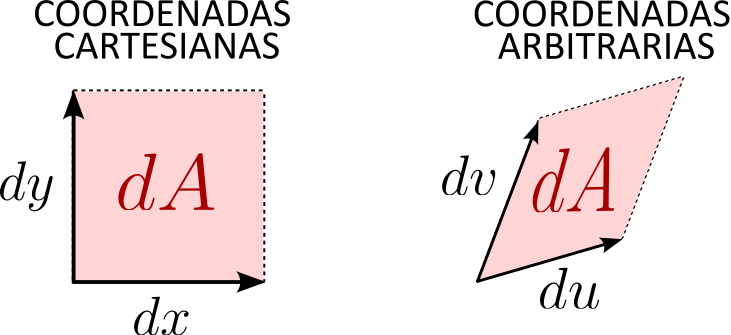
\includegraphics[scale=.4]{FOTOS/elem_area.png}
\end{center}
En el caso de las coordenadas cartesianas, el elemento diferencial de área se calculará como $\odif{A}=\odif{x}\odif{y}$. Cuando usemos coordenadas arbitrarias, veremos que necesitaremos un 'determinante' que transforme el elemento de área cartesiano.\\

Sea una superficie con una carta local,
\begin{align*}
    \mathbf{x}:U\subseteq\mathbb{R}^2&\longrightarrow V \cap S\\
                        (u^1,u^2)&\longmapsto \mathbf{x}(u^1,u^2);
\end{align*}
y $\Omega \subset U$ es un dominio cerrado de $U$. Bajo estas condiciones, el área de $\mathbf{x}(\Omega)=\Sigma$ es:\\
\begin{wrapfigure}{r}{0.3\textwidth}
    \centering
    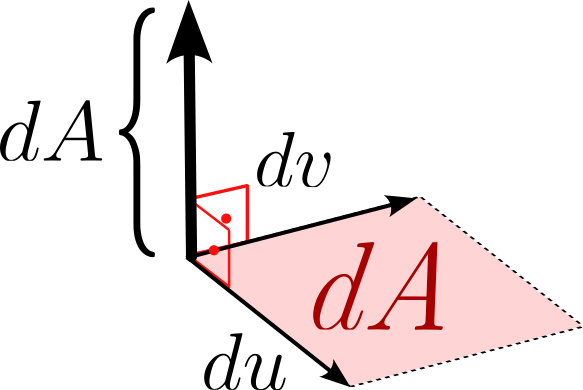
\includegraphics[scale=.3]{FOTOS/jacobiano.png}
\end{wrapfigure}
$$
A(\Sigma)=\int \!\!\!\!\int _\Omega \left | \left | \pdv{\mathbf{x}}{u^1}\wedge \pdv{\mathbf{x}}{u^2} \right | \right |\odif{u^1}\odif{u^2}
$$
En este caso, lo que actúa para modificar el elemento diferencial de área es el módulo del producto vectorial de los dos vectores de nuestra base de $T_p(S)$. Sustituyendo sus expresiones en el integrando, llegamos a que:
$$
A(\Sigma)=\int \!\!\!\!\int _\Omega ||\mathbf{x}_1\wedge \mathbf{x}_2||\odif{u^1}\odif{u^2}
$$

Ahora queda calcular el módulo de ese vector,
\begin{equation*}
    \begin{split}
        ||\mathbf{x}_1\wedge \mathbf{x}_2||^2&=(\mathbf{x}_1\wedge \mathbf{x}_2)\cdot (\mathbf{x}_1\wedge \mathbf{x}_2)\\
                                     &=||\mathbf{x}_1||^2||\mathbf{x}_2||^2 \sin ^2 \theta = ||\mathbf{x}_1||^2 ||\mathbf{x}_2||^2 (1-\cos ^2 \theta)\\
                                     &=g_{11}\cdot g_{22}(1-\cos ^2 \theta)=g_{11}g_{22}-g_{12}g_{21}\equiv g \ \left (=\det{g_{\alpha\beta}}\right )
    \end{split}
\end{equation*}
Y finalmente:
$$
\boxed{A(\Sigma)=\int \!\!\!\!\int _\Omega \sqrt{g}\odif{u^1}\odif{u^2}}
$$
\section{Vectores contravariantes y covariantes}
Ahora nos planteamos qué tipo de reparametrizaciones podemos usar.

Es importante recordar que las longitudes \emph{no cambian} bajo reparametrizaciones. El tensor métrico que hemos calculado servirá como regla de medida, e independientemente del convenio que usemos, estas longitudes siempre serán las mismas.
$$
t\xlongrightarrow{\text{difeomorf.}}\Bar{t}(t)
$$
\subsection{Reparametrizaciones}
Sea $\vec{\Phi}$ un difeomorfismo de $\Bar{U}$ en $U$:
\begin{align*}
    \vec{\Phi}:\Bar{U}\subseteq \mathbb{R}^2 &\longrightarrow U\subseteq \mathbb{R}^2\\
    (\Bar{u}^1,\Bar{u}^2)&\longmapsto \left ( \Bar{u}^1(u^1,u^2),\Bar{u}^2(u^1,u^2) \right )
\end{align*}

$\vec{\Phi}$ es un \emph{homeomorfismo} diferenciable, con función inversa diferenciable. Es decir, en la región de intersección entre dos cartas de una superficie, la función de transición tiene que ser un difeomorfismo. Se cumple por tanto que:
\begin{enumerate}
    \item[I)] $\vec{\Phi}:\Bar{U}\longrightarrow U$ es \emph{biyectiva}.
    \item[II)] $\vec{\Phi}:\Bar{U}\longrightarrow U$ es diferenciable ($\vec{\Phi}\in C^\infty$).
    \item[III)] $\vec{\Phi}^{-1}:U\longrightarrow \Bar{U}$ es diferenciable (de clase $C^\infty$).
\end{enumerate}

En notación más compacta, escribiremos el difeomorfismo como:
$$
\boxed{u^\alpha=u^\alpha (\Bar{u}^\beta)} \ , \ \text{con }\alpha,\beta=1,2
$$

El jacobiano de la \emph{transformación directa} es el determinante:
$$
D=\det{\left ( \pdv{u^\alpha}{\Bar{u}^\beta} \right )}
$$
y el de la \emph{transformación inversa} es:
$$
\Bar{D}=\det{\left ( \pdv{\Bar{u}^\alpha}{u^\beta} \right )} \ ;
$$
ambos con $\alpha,\beta=1,2$. Además, por el \emph{Teorema de la función inversa}, se cumple que:
$$
\pdv{u^\alpha}{\Bar{u}^\beta}\cdot \pdv{\Bar{u}^\beta}{u^\gamma }=\delta ^\alpha {}_\gamma  \xleftrightarrow{\text{matric.}} D\cdot \Bar{D}=\mathbb{1}
$$

\begin{mybox}
    \underline{Ejemplo C:} $u^1(\Bar{u}^1,\Bar{u}^2)=e^{\Bar{u}^1+\Bar{u}^2}\ , \ u^2(\Bar{u}^1,\Bar{u}^2)=e^{\Bar{u}^1-\Bar{u}^2}$\\

    $\hookrightarrow$ La transformación inversa es: $ \left \{
    \begin{array}{ccc}
         \Bar{u}^1&=&1/2\log(u^1\cdot u^2)  \\
         \Bar{u}^2&=&1/2\log(u^1/u^2) 
    \end{array} \right . \ \left (\Bar{u}^\alpha (u^\beta)\right )
    $\\
    $
    \rightarrow D^\alpha _\beta =\left ( \pdv{u^\alpha}{\Bar{u}^\beta} \right )=\left ( 
    \begin{array}{cc}
         e^{\Bar{u}^1+\Bar{u}^2}&e^{\Bar{u}^1+\Bar{u}^2}  \\
         e^{\Bar{u}^1-\Bar{u}^2}&-e^{\Bar{u}^1-\Bar{u}^2} 
    \end{array}
    \right ) = \left ( 
    \begin{array}{cc}
         u^1&u^1  \\
         u^2&-u^2 
    \end{array}
    \right )\implies D=-2u^1u^2
    $\\
    $
    \rightarrow \Bar{D}^\alpha_ \beta =\left ( \pdv{\Bar{u}^\alpha}{u^\beta} \right )= \cdots =\left ( 
    \begin{array}{cc}
         1/(2u^1)&1/(2u^2)  \\
         1/(2u^1)&-1/(2u^2) 
    \end{array}
    \right ) \implies \Bar{D}=-\frac{1}{2u^1u^2}
    $\\
    $
    \implies \left ( \pdv{u^\alpha}{\Bar{u}^\beta} \right ) \left ( \pdv{\Bar{u}^\alpha}{u^\beta} \right )=\delta ^\alpha {}_\beta  \qquad(D^\alpha _\beta \Bar{D}^\beta _\gamma =\delta ^\alpha {}_\gamma  )
    $
\end{mybox}

Veamos cómo se relacionan las bases en el plano tangente $T_p(S)$ tras una reparametrización.
$$
\Bar{\mathbf{x}}(\Bar{u}^1,\Bar{u}^2)=\mathbf{x}\left (u^1(\Bar{u}^1,\Bar{u}^2),u^2(\Bar{u}^1,\Bar{u}^2)\right )
$$
En notación compacta, diremos que $\Bar{\mathbf{x}}(\Bar{u}^\beta)=\mathbf{x}(u^\alpha (\Bar{u}^\beta))$. Cada carta $(U,\mathbf{x}(u^\alpha))$ y $(\Bar{U},\Bar{\mathbf{x}}(\Bar{u}^\beta))$ tiene un plano tangente, o más bien, una base de vectores del plano tangente $T_p(S)$.
$$
\left \{ \mathbf{x}_1=\pdv{\mathbf{x}}{u^1},\mathbf{x}_2=\pdv{\mathbf{x}}{u^2} \right \} \ , \ \left \{ \Bar{\mathbf{x}}_1=\pdv{\Bar{\mathbf{x}}}{\Bar{u}^1}, \Bar{\mathbf{x}}_2=\pdv{\Bar{\mathbf{x}}}{\Bar{u}^2} \right \}
$$

Busquemos la relación entre $\mathbf{x}_\alpha$ y $\mathbf{x}_\beta$. Por la regla de la cadena,
$$
\Bar{\mathbf{x}}_\beta = \pdv{\Bar{\mathbf{x}}}{\Bar{u}^\beta}=\pdv{\mathbf{x}}{u^\alpha}\cdot \pdv{u^\alpha}{\Bar{u}^\beta}=\pdv{u^\alpha}{\Bar{u}^\beta}\cdot \pdv{\mathbf{x}}{u^\alpha}=\pdv{u^\alpha}{\Bar{u}^\beta}\mathbf{x}_\alpha
$$
Es decir:
$$
\boxed{\Bar{\mathbf{x}}_\beta =\pdv{u^\alpha}{\Bar{u}^\beta}\mathbf{x}_\alpha}
$$

Esta es la relación entre las bases $\{ \mathbf{x}_\alpha  \}$ y $\{ \Bar{\mathbf{x}}_\beta \}$ tras el cambio de coordenadas. $\left ( \pdv{u^\alpha}{\Bar{u}^\beta} \right )$ es la \emph{matriz de cambio de base}. Su transformación inversa es:
$$
\boxed{\mathbf{x}_\alpha=\pdv{\Bar{u}^\beta}{u^\alpha}\Bar{\mathbf{x}}_\beta}
$$
\begin{mybox}
    \begin{center}
        \textbf{ORIENTABILIDAD}
    \end{center}
    Para que las cartas $(U,\mathbf{x}(u^\alpha))$ y $(\Bar{U},\Bar{\mathbf{x}}(\Bar{u}^\beta))$ describan la misma superficie y den lugar al mismo plano tangente (con el vector perpendicular en la misma orientación), se tiene que cumplir que
    $$
    D=\det{\pdv{u^\alpha}{\Bar{u}^\beta}}>0
    $$
    Si no lo cumple, hacemos el cambio $\Bar{u}^1\leftrightarrow \Bar{u}^2$.
\end{mybox}

Resumiendo, bajo difeomorfismos, tenemos las siguientes \emph{reglas de cambio de base}.
\begin{mybox}
    \begin{center}
        \textbf{CAMBIO DE BASE}
    \end{center}
    Bajo difeomorfismos (por la regla de la cadena), tenemos que, en las bases $\{\mathbf{x}_\alpha\}$ y $\{ \Bar{\mathbf{x}}_\beta \}$.
    $$
    \mathbf{x}_\alpha=\pdv{\Bar{u}^\beta}{u^\alpha}\Bar{\mathbf{x}}_\beta \qquad  \qquad \Bar{\mathbf{x}}_\beta=\pdv{u^\alpha}{\Bar{u}^\beta}\mathbf{x}_\alpha
    $$
\end{mybox}

\subsection{Leyes de transformación}
Sea $\mathbf{v}\in T_p(S)$. Entonces, $\mathbf{v}=v^\alpha \mathbf{x}_\alpha$ (con el convenio de Einstein), o bien, si decidimos transformarlo a otras coordenadas, $\mathbf{v}=\Bar{v}^\alpha \Bar{\mathbf{x}}_\alpha$. $v^\alpha$ y $\Bar{v}^\alpha$ son las componentes del vector entre las bases $\{ \mathbf{x}_\alpha \}$ y $\{ \Bar{\mathbf{x}}_\alpha \}$. Usando la información del cambio de base visto anteriormente, decimos que:
\begin{gather*}
    \mathbf{v}=v^\alpha \mathbf{x}_\alpha =v^\alpha \pdv{\Bar{u}^\beta}{u^\alpha} \Bar{\mathbf{x}}_\beta=\Bar{v}^\beta \Bar{\mathbf{x}}_\beta \\
    \boxed{\Bar{v}^\beta=\pdv{\Bar{u}^\beta}{u^\alpha}v^\alpha}
\end{gather*}
Esta es la \emph{ley de transformación de las componentes contravariantes} de un vector (veremos más adelante por qué las llamaremos contravariantes). De hecho, las relaciones de cambio de base serán las leyes de transformación de los vectores covariantes de la base en $T_p(S)$.\\

\begin{wrapfigure}{l}{.4\textwidth}
    \centering
    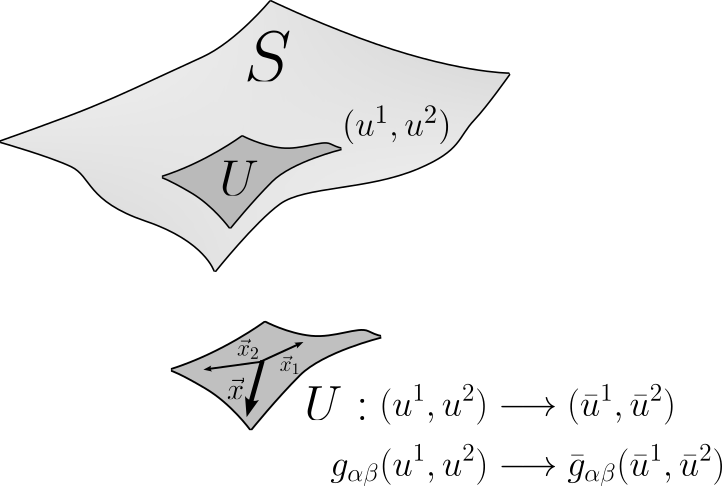
\includegraphics[scale=.45]{FOTOS/forma_fundamental_trans.png}
\end{wrapfigure}

Veamos ahora cuál es la regla de transformación de la primera forma fundamental bajo reparametrizaciones (con difeomorfismos).
\begin{align*}
    g_{\alpha \beta}      =\mathbf{x}_\alpha \cdot \mathbf{x}_\beta \longrightarrow    
    \Bar{g}_{\alpha \beta}&=\Bar{\mathbf{x}}_\alpha \cdot \Bar{\mathbf{x}}_\beta\\
                          &=\left ( \pdv{u^\mu}{\bar{u}^\alpha}\mathbf{x}_\mu  \right ) \cdot \left ( \pdv{u^\nu}{\bar{u}^\beta}\mathbf{x}_\nu  \right )\\
                          &=\pdv{u^\mu}{\bar{u}^\alpha} \pdv{u^\nu}{\bar{u}^\beta} \mathbf{x}_\mu \cdot \mathbf{x}_\nu\\
                          &=\pdv{u^\mu}{\bar{u}^\alpha} \pdv{u^\nu}{\bar{u}^\beta} g_{\mu \nu}
\end{align*}
$$
\boxed{\Bar{g}_{\alpha \beta}=\pdv{u^\mu}{\bar{u}^\alpha} \pdv{u^\nu}{\bar{u}^\beta} g_{\mu \nu}}
$$
\WFclear
\begin{itemize}
    \item \emph{Comentario}: Los índices $\alpha,\beta,\mu,\nu$ que aparecen \emph{abajo} son índices \emph{covariantes.} 
\end{itemize}

Bajo difeomorfismos, el determinante de la primera forma fundamental se transforma según la siguiente ley:
\begin{equation*}
    \begin{split}
        g&=\det{g_{\alpha \beta}} =g_{11}g_{22}-g_{12}g_{21}\\
\implies   \Bar{g}&=\Bar{g}_{11}\Bar{g}_{22}-\Bar{g}_{12}\Bar{g}_{21} \\
& =\left ( \pdv{u^\mu}{\bar{u}^1} \pdv{u^\nu}{\bar{u}^1} \right )g_{\mu \nu}\cdot \left ( \pdv{u^\rho}{\bar{u}^2} \pdv{u^\sigma}{\bar{u}^2} \right )g_{\rho \sigma} - \left ( \pdv{u^\mu}{\bar{u}^1} \pdv{u^\nu}{\bar{u}^2} \right )g_{\mu \nu}\cdot \left ( \pdv{u^\rho}{\bar{u}^2} \pdv{u^\sigma}{\bar{u}^1} \right )g_{\rho \sigma} \\
         &=g\cdot D^2 \quad , \quad \text{con $D$ el determinante jacobiano}
    \end{split}
\end{equation*}
$$
\boxed{\Bar{g}=gD^2}
$$

Y, por lo tanto, la ley de transformación de $g$ asegura que el área de una superficie sea invariante bajo reparametrizaciones por un difeomorfismo.
\begin{align*}
    A(\Sigma)      &=\int \! \! \! \! \int _\Omega \sqrt{g}\odif{u^1}\odif{u^2}\\
    \Bar{A}(\Sigma)&=\int \! \! \! \! \int _{\Bar{\Omega}} \sqrt{\Bar{g}} \odif{\Bar{u}^1} \odif{\Bar{u}^2} =\int \! \! \! \! \int _\Omega \sqrt{D^2 g}\ |\Bar{D}|\odif{u^1}\odif{u^2}=\int \! \! \! \! \int _\Omega \sqrt{g}\odif{u^1}\odif{u^2}=A(\Sigma) \ \smiley
\end{align*}

\subsection{Base dual. Componentes covariantes de un vector}
Dado el plano tangente a la superficie $T_p(S)$, una base de dicho plano es $\left \{ \mathbf{x}_1=\pdv{\mathbf{x}}{u^1},\mathbf{x}_2=\pdv{\mathbf{x}}{u^2} \right \}\equiv B$. Una base del espacio vectorial \emph{dual} a $T_p(S)$, $T_p^*(S)$, será:
$$
\left \{ \mathbf{x}^{1*},\mathbf{x}^{2*} \right \}=\left \{ \mathbf{x}^1,\mathbf{x}^2 \right \}.
$$

En esta base, los vectores tienen \emph{superíndices} en vez de subíndices. y cumplen que:
$$
\mathbf{x}^\alpha \cdot \mathbf{x}_\beta =\delta ^\alpha {}_\beta 
$$

\begin{mybox}
    \underline{Ejemplo D:} En $\mathbb{R}^2$, $\left \{ \mathbf{x}_1=(2,0),\mathbf{x}_2=\left ( \frac{1}{\sqrt{2}},\frac{1}{\sqrt{2}} \right ) \right \}$. La base dual debe cumplir que:
    \begin{itemize}
        \item $\mathbf{x}^2$ debe ser ortogonal a $\mathbf{x}_1$ y paralelo a $\mathbf{x}_2$.\\
        $\implies \mathbf{x}^2$ es de la forma $\mathbf{x}^2=(0,a) \ (\mathbf{x}^2\cdot \mathbf{x}_1=0)$\\
        $\implies a=\sqrt{2}$ (por la condición $\mathbf{x}^2\cdot \mathbf{x}_2=1$)
        $$
        \iff \mathbf{x}^2=\left (0,\sqrt{2} \right )
        $$

        \item $\mathbf{x}^1$ debe ser ortogonal a $\mathbf{x}_2$ y paralelo a $\mathbf{x}_1$.\\
        $\implies \mathbf{x}^1=(b,-b)$ ($\mathbf{x}^1\cdot \mathbf{x}_2=0$)\\
        $\implies b=1/2$ ($\mathbf{x}^1\cdot \mathbf{x}_1=1$)
        $$
        \iff \mathbf{x}^1=\left ( \frac{1}{2},-\frac{1}{2} \right )
        $$
    \end{itemize}
    $$
    B^*=\left \{ \mathbf{x}^1=\left ( \frac{1}{2},-\frac{1}{2} \right ),\mathbf{x}^2=\left (0,\sqrt{2} \right ) \right \}
    $$
    que es una base de $\left (\mathbb{R}^2\right )^*=\mathbb{R}^2$ (espacios auto-duales).
\end{mybox}
La idea de introducir la base dual es para poder calcular las componentes \emph{contravariantes} de un vector mediante productos escalares. Supongamos que tenemos $\mathbf{v}\in T_p(S)$, $\left \{ \mathbf{x}_\alpha \right \}$ una base de ese espacio y $\{ \mathbf{x}^\beta  \}$ del espacio dual.
\begin{gather*}
    \mathbf{v}=v^\alpha \mathbf{x}_\alpha \\
    \mathbf{v} \cdot \mathbf{x}^\beta=(v^\alpha \mathbf{x}_\alpha) \cdot \mathbf{x}^\beta =v^\alpha (\mathbf{x}_\alpha \cdot \mathbf{x}^\beta)=v^\alpha \delta _\alpha {}^\beta =v^\beta
\end{gather*}
$$
\boxed{\mathbf{v}\cdot \mathbf{x}^\beta=v^\beta}
$$
Veamos ahora la relación entre las bases $B$ y $B^*$. Definiremos para eso la inversa de la primera forma fundamental como:
$$
g_{\alpha \beta }^{-1}=g^{\alpha \beta } \qquad \qquad \text{como matrices, }g_{\alpha \beta} \cdot g^{\beta \gamma}=\delta ^\gamma {}_\alpha
$$

Los vectores de esta base dual $B^*$, $\{ \mathbf{x}^\alpha \}$ cumplen entonces que 
\begin{equation*}
    \begin{split}
        \mathbf{x}^\alpha=g^{\alpha \beta} \mathbf{x}_\beta \longrightarrow \mathbf{x}^\alpha \cdot \mathbf{x}_\beta &=g^{\alpha \beta}\mathbf{x}_\rho \cdot \mathbf{x}_\beta\\
        &=g^{\alpha \rho}g_{\rho \beta} =\delta ^\alpha {}_\beta 
    \end{split}
\end{equation*}

Las componentes de un vector en la base dual $B^*$ se denominan, por tanto, \emph{componentes covariantes} del vector, y se tiene que 
$$
\mathbf{v}=v^\alpha \mathbf{x}_\alpha =v_\beta \mathbf{x}^\beta =v_\beta g^{\alpha \rho}\mathbf{x}_\rho 
$$
$$
\boxed{v^\alpha =v_\beta g^{\beta \alpha} =g^{\alpha\beta}v_\beta}
$$
Es decir, $g^{\alpha \beta}$ permite subir índices. De forma análoga, $g_{\alpha \beta}$ permite bajar índices,
$$
v_\alpha =g_{\alpha \beta} v^\beta
$$
\begin{mybox}
    \begin{center}
        \textbf{COMPONENTES COVARIANTES Y CONTRAVARIANTES}
    \end{center}
    Las componentes \textbf{contravariantes} de $\mathbf{v}$ son $v^\alpha$. Las componentes \textbf{covariantes} de $\mathbf{v}$ son $v_\alpha$. Por convenio, usamos la notación \emph{covariante} para denotar \emph{subíndices}; y \emph{contravariante} para denotar \emph{superíndices}. La relación entre componentes covariantes y contravariantes es:
    \begin{gather*}
        v^\alpha=g^{\alpha\beta}v_\beta \qquad \qquad v_\alpha =g_{\alpha \beta} v^\beta
    \end{gather*}
    con $g^{\alpha \beta }=g_{\alpha \beta }^{-1} $ la inversa de la primera forma fundamental.
\end{mybox}
Los nombres se deben a la manera en la que se transforman bajo cambios de coordenadas o difeomorfismos.\\

Sea $u^\alpha =u^\alpha (\Bar{u}^\beta)$ el cambio de coordenadas. Por la regla de la cadena:
$$
\Bar{\mathbf{x}}_\alpha =\pdv{u^\beta }{\Bar{u}^\alpha }\mathbf{x}_\beta 
$$
$
\implies
$ Los vectores covariantes se transforman con la matriz $\pdv{u^\beta }{\Bar{u}^\alpha}$

Las componentes contravariantes $\Bar{v}^\alpha =\pdv{\Bar{u}^\alpha }{u^\beta }v^\beta$ se transforman con la matriz inversa.
$$
\underbrace{\pdv{u^\beta }{\Bar{u}^\alpha }}_{\text{\parbox{4cm}{\centering
Matriz directa\\ Prefijo 'co'}}} \qquad  \underbrace{\pdv{\Bar{u}^\alpha }{u^\beta}}_{\text{\parbox{4cm}{\centering
Matriz inversa\\ Prefijo 'contra'}}}
$$

Las componentes covariantes se transforman con la primera forma fundamental transformada, $\Bar{g}_{\alpha \beta}$, como sigue:
\begin{equation*}
    \begin{split}
        \Bar{v}_\alpha=\Bar{g}_{\alpha \beta} \Bar{v}^\beta &=\pdv{u^\rho }{\Bar{u}^\alpha }\pdv{u^\sigma }{\Bar{u}^\beta }g_{\rho \sigma} \Bar{v}^\beta=\pdv{u^\rho }{\Bar{u}^\alpha }\pdv{u^\sigma }{\Bar{u}^\beta}g_{\rho \sigma }\pdv{\Bar{u}^\beta }{u^\gamma }v^\gamma\\
        &= \pdv{u^\rho }{\Bar{u}^\alpha }\delta ^\sigma{}_\gamma  g_{\rho \sigma }v^\gamma =\pdv{u^\rho }{\Bar{u}^\alpha } v_\rho =\pdv{u^\beta }{\Bar{u}^\alpha }v_\beta
    \end{split}
\end{equation*}
$$
\boxed{\Bar{v}_\alpha =\pdv{u^\beta }{\Bar{u}^\alpha }v_\beta}
$$
\begin{mybox}
    \begin{center}
        \textbf{LEYES DE TRANSFORMACIÓN DE COMPONENTES}
    \end{center}
    $$
    \begin{array}{ccc}
         \text{\textbf{Matriz directa}}&& \text{\textbf{Matriz inversa}} \\
         \cfrac{\partial u^\beta }{\partial \Bar{u}^\alpha }&&\cfrac{\partial \Bar{u}^\alpha }{\partial u^\beta}\\
         \Bar{v}_\alpha =\cfrac{\partial u^\beta }{\partial \Bar{u}^\alpha }v_\beta&&\Bar{v}^\alpha =\cfrac{\partial \Bar{u}^\alpha }{\partial u^\beta }v^\beta 
    \end{array} 
    $$
\end{mybox}

En $T_p(S)$ tenemos un producto escalar. Si $\mathbf{v},\mathbf{w}\in T_p(S)$, entonces:
\begin{equation*}
    \begin{split}
        \left . \begin{array}{ccc}
             \mathbf{v}&=&v^\alpha \mathbf{x}_\alpha   \\
             \mathbf{w}&=&w^\beta \mathbf{x}_\beta  
        \end{array} \right \} \longrightarrow \mathbf{v}\cdot \mathbf{w}&=v^\alpha w^\beta \mathbf{x}_\alpha \mathbf{x}_\beta =v^\alpha w^\beta g_{\alpha \beta}\\
        &=v_\beta w^\beta =v^\alpha w_\alpha 
    \end{split}
\end{equation*}

La contracción de los índices covariantes y contravariantes de las componentes de un vector da lugar a una cantidad \emph{escalar} (que más adelante veremos que es invariante).

\subsection{Tensores}
El cambio de índices o componentes covariantes a contravariantes y viceversa se lleva a cabo mediante la inversa de la primera forma fundamental, o mediante la propia primera forma fundamental. \\

$\rightarrow $ BAJAR ÍNDICES: Contravariante $\to $ covariante\\
$$
v_\alpha =g_{\alpha \beta }v^\beta
$$

$\rightarrow $ SUBIR ÍNDICES: Covariante $\to $ contravariante\\
$$
v^\alpha =g^{\alpha \beta} v_\beta 
$$

La primera forma fundamental $g_{\alpha \beta} =\mathbf{x}_\alpha \cdot \mathbf{x}_\beta $ con dos índices no repetidos (o libres) es un ejemplo de \emph{tensor} de segundo orden.
\begin{itemize}
    \item El número de índices del tensor indica su \emph{orden tensorial}.
    \item Si los índices están \emph{abajo}, como $g_{\alpha \beta}$, el tensor se dice \emph{dos veces covariante}.
    
    $\hookrightarrow$Covariante dos veces: $ \Bar{g}_{\alpha \beta} = \pdv{u^\mu }{\Bar{u}^\alpha }\pdv{u^\nu }{\Bar{u}^\beta }g_{\mu \nu}$ 
    \item Si los índices están \emph{arriba}, como $g^{\alpha \beta} $, el tensor se dice \emph{dos veces contravariante}.
    
    $\hookrightarrow $Contravariante dos veces: $\Bar{g}^{\alpha \beta}=\pdv{\Bar{u}^\alpha }{u^\mu }\pdv{\Bar{u}^\beta }{u^\nu }g^{\mu \nu}$

    \item Cuando un tensor tiene tanto índices covariantes como índices contravariantes, se conoce como tensor \emph{mixto} (que puede ser $k$ veces covariante y $j$ veces contravariante).\\

    $\hookrightarrow$ Para la primera forma fundamental:
    $$
    \Bar{g}^\alpha{} _\beta=\pdv{\Bar{u}^\alpha }{u^\mu} \pdv{u^\nu }{\Bar{u}^\beta }g^\mu {}_\nu \longrightarrow g^\mu{} _\nu =g^{\mu \rho }g_{\rho \nu }=\delta ^\mu{}_\nu 
    $$

    \item Los tensores con más de dos índices son tensores de orden superior.
\end{itemize}
\section{Geometría riemanniana}
La geometría riemanniana extiende la noción de superficie a lo que se conoce como \emph{variedades} de dimensión $n$ (las superficies son variedades bidimensionales). Localmente, en una variedad diferenciable de dimensión $n$, podemos introducir un sistema de coordenadas $(u^1,u^2,\ldots , u^n)$ y un conjunto de $n^2$ funciones $g_{\alpha \beta} (u^1,u^2,\ldots, u^n)$, donde $\alpha ,\beta=1,2,\ldots , n$, y ordenadas matricialmente; que cumplen lo siguiente:
\begin{enumerate}
    \item[I)] La matriz es simétrica, $g_{\alpha \beta}=g_{\beta \alpha}$
    \item[II)] La matriz es definida positiva, es decir, todos sus menores son positivos.
    \item[III)] Al cambiar de carta por una reparametrización,
    $$
    \Bar{g}_{\alpha \beta}=\pdv{u^\mu }{\Bar{u}^\alpha }\pdv{u^\nu }{\Bar{u}^\beta }g_{\mu \nu}
    $$
\end{enumerate}
(El segundo requerimiento puede no cumplirse en el caso de encontrarnos en geometría pseudo-riemanniana, como en Relatividad General.)\\

En geometría riemanniana, las funciones $g_{\alpha \beta} $ se conocen como \emph{métrica} o \emph{tensor métrico}.
\begin{gather*}
    \odif{S^2}=g_{\alpha \beta} \odif{u^\alpha}\odif{u^\beta}\\
    \alpha ,\beta =1,2,\ldots, n
\end{gather*}

Para el caso en el que la dimensión $n=2$, recuperamos las variedades o superficies bidimensionales. De forma general, el tensor métrico $g_{\alpha \beta}$ representa el \emph{elemento de línea} de la variedad, $\odif{S^2}=g_{\alpha \beta} \odif{u^\alpha }\odif{u^\beta}$.

\begin{wrapfigure}{r}{.37\textwidth}
    \centering
    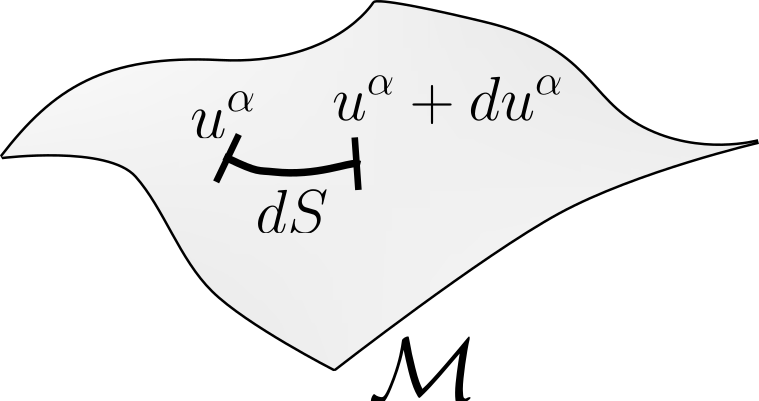
\includegraphics[scale=.3]{FOTOS/manifold.png}
\end{wrapfigure}

Dada la variedad $\mathcal{M}$ de dimensión $n$, para construir el espacio $T_p(\mathcal{M})$, de dimensión $n$, necesitamos las derivadas direccionales $\mathbf{x}_\alpha $, con $\alpha =1,2,\ldots ,n$. 

En el caso de las superficies bidimensionales conocemos $\mathbf{x}(u^1,u^2)$, esto es, la carta local de la superficie $S$. En general, para variedades $\mathcal{M}$ no se conoce $\mathbf{x}(u^1,\ldots , u^n)$.\\

Como no disponemos de $\mathbf{x}$, lo eliminaremos de la definición de las derivadas direccionales.
$$
\mathbf{x}_\alpha =\left .\pdv{}{u^\alpha }\right |_{(u^1,u^2,\ldots,u^n)}
$$
De este modo: $\mathbf{v}\in T_p(\mathcal{M}) \ , \ \mathbf{v}=v^\alpha \mathbf{x}_\alpha =v^\alpha \partial _\alpha $ con $\alpha =1,\ldots ,n$ y $\partial_\alpha =\pdv{}{u^\alpha }$.\\

Con esta definición, $v^\alpha $ son las componentes contravariantes del vector $\mathbf{v}\in T_p(\mathcal{M})$. Para verlo, basta con cambiar de parametrización en $\mathcal{M}$, $(\Bar{u}^1,\Bar{u}^2,\ldots ,\Bar{u}^n)\longrightarrow (u^1,u^2,\ldots , u^n)$.
\begin{align*}
    \mathbf{v}&=v^\alpha \mathbf{x}_\alpha =v^\alpha \partial_\alpha =v^\alpha \pdv{}{u^\alpha }\\
    \downarrow&\\
    \Bar{\mathbf{v}}&=\Bar{v}^\beta \Bar{\mathbf{x}}_\beta =\Bar{v}^\beta \Bar{\partial}_\beta =\Bar{v}^\beta \pdv{}{\Bar{u}^\beta }
\end{align*}
Como $\mathbf{v}=\Bar{\mathbf{v}}$:
\begin{gather*}
    v^\alpha \partial_\alpha =v^\alpha \pdv{}{u^\alpha }=v^\alpha \pdv{\Bar{u}^\beta }{u^\alpha }\pdv{}{\Bar{u}^\beta }=\pdv{\Bar{u}^\beta }{u^\alpha } v^\alpha \Bar{\partial}_\beta \\
    \boxed{\Bar{v}^\beta =\pdv{\Bar{u}^\beta }{u^\alpha } v^\alpha }
\end{gather*}
que es la ley de transformación de las componentes contravariantes de $\mathbf{v}$. \\

Para una variedad $\mathcal{M}$ de dimensión $n$, la base dual del espacio tangente, $\{ \mathbf{x}^\alpha  \}$, se construye a través del producto interno (o escalar) definido en $T_p(\mathcal{M})$. Para asegurar que se cumple que $\langle \mathbf{x}^\alpha , \mathbf{x}_\beta \rangle =\delta ^\alpha {}_\beta  $ (el producto que define el espacio vectorial dual), basta con tomar los $\mathbf{x}^\alpha $ como:
$$
\boxed{\mathbf{x}^\alpha =\odif{u^\alpha }} \ ,
$$
que son los diferenciales de línea, conocidos también como 1-formas diferenciables de Cartan. Los elementos de la base dual, $\{ \odif{u^\alpha } \}$, cumplen que:
$$
\Bar{\mathbf{x}}^\alpha =\odif{\Bar{u}^\alpha }=\pdv{\Bar{u}^\alpha }{u^\beta }\odif{u^\beta} =\pdv{\Bar{u}^\alpha }{u^\beta } \mathbf{x}^\beta \ ,
$$
que es la ley de transformación contravariante.
\begin{mybox}
    $\left \{ \begin{array}{cccc}
        \mathbf{x}_\alpha  &=&\partial_\alpha&  \\
        &&&\text{con }\alpha =1,\ldots ,n\\
         \mathbf{x}^\alpha &=&\odif{u^\alpha }&
    \end{array} \right | \ \text{\parbox{8cm}{El espacio dual a $T_p(\mathcal{M})$, cuya base es $\{ \mathbf{x}^\alpha  \}=\{ \odif{u^\alpha } \}$, se conoce como el espacio \textbf{cotangente} a $\mathcal{M}$ en el punto $P$.}}$ 
\end{mybox}

De esta forma, para la variedad $\mathcal{M}$, el producto escalar en $T_p(\mathcal{M})$ está definido como:
\begin{equation*}
    \begin{split}
        \begin{array}{c}
             \mathbf{v}=v^\alpha \mathbf{x}_\alpha   \\
             \mathbf{w}=w^\beta \mathbf{w}_\beta
        \end{array} \ ; \ \mathbf{v},\mathbf{w}\in T_p(\mathcal{M}):\mathbf{v}\cdot \mathbf{w}&=v_\alpha w^\alpha =v^\beta w_\beta =g_{\alpha \beta }v^\alpha w^\beta\\
        \mathbf{v}&=v^\alpha \mathbf{x}_\alpha =v_\alpha \mathbf{x}^\alpha \\
      \text{Donde hemos usado}\quad   \mathbf{w}&=w^\beta \mathbf{x}_\beta =w_\beta \mathbf{x}^\beta \\
        v_\alpha &=g_{\alpha \beta }v^\beta \ \text{(subir y bajar índices)}
    \end{split}
\end{equation*}

El espacio de 1-formas en el espacio cotangente y las derivadas direccionales en el espacio tangente permiten construir tensores como aplicaciones, en base a su regla o ley de transformación. \\
De acuerdo con su ley de transformación, podemos clasificar los tensores de la siguiente manera:

\begin{enumerate}
    \item[(i)] \underline{Escalares:} Una aplicación es un escalar si $h=\Bar{h}$. Explícitamente:
    $$
    \Bar{h}(\Bar{u}^\alpha )=h(u^\alpha)
    $$
    Un escalar es una cantidad puramente geométrica e invariante frente al sistema de coordenadas elegido.

    \item[(ii)] \underline{Vectores o tensores de orden uno:} \\
    En componentes contravariantes$\longrightarrow \Bar{v}^\beta =\pdv{\Bar{u}^\beta }{u^\alpha }v^\alpha $\\
    En componentes covariantes    $\longrightarrow \Bar{u}_\beta =\pdv{u^\beta }{\Bar{u}^\alpha }v_\alpha $\\

    \item[(iii)] \underline{Tensores de orden dos:} \\
    Dos veces contravariante $\longrightarrow \Bar{a}^{\alpha \beta} =\pdv{\Bar{u}^\alpha }{u^\mu }\pdv{\Bar{u}^\beta }{u^\nu}a^{\mu \nu}$\\
    Dos veces covariantes$\longrightarrow \Bar{a}_{\alpha \beta} =\pdv{u^\mu}{\Bar{u}^\alpha }\pdv{u^\nu }{\Bar{u}^\beta }a_{\mu \nu}$\\
    Tensor mixto (1 covariante 1 contravariante)$\longrightarrow \Bar{a}^\alpha {}_\beta =\pdv{\Bar{u}^\alpha }{u^\mu }\pdv{u^\nu }{\Bar{u}^\beta }a^\mu {}_\nu $

    \item[(iv)] \underline{Tensor de orden $r+s$ (r veces covariante, s veces contravariante)}:
    $$
    \Bar{h}_{\alpha _1,\ldots ,\alpha _r}{}^{\beta_1,\ldots ,\beta_s}=\pdv{u^{\mu_1}}{\Bar{u}^{\alpha _1}}\cdots \pdv{u^{\mu_r}}{\Bar{u}^{\alpha _r}}\pdv{\Bar{u}^{\beta _1}}{u^{\nu_1}}\cdots \pdv{\Bar{u}^{\beta _s}}{u^{\nu_s}} h_{\mu_1,\ldots , \mu _r}{}^{\nu_1, \ldots , \nu_s} 
    $$
\end{enumerate}
\section{Fundamentos del cálculo tensorial}
\begin{itemize}
   \item La \emph{suma} de tensores está definida para tensores del mismo tipo (con la misma disposición de índices).

    Por ejemplo: $a^\mu {}_\nu +b^\mu {}_\nu =c^\mu {}_\nu $.\\

   \item El \emph{producto tensorial} está definido para tensores de cualquier tipo.

    Por ejemplo: $a^\mu {}_\nu b^\rho =c^\mu {}_\nu {}^\rho \longrightarrow \text{\parbox{7.5cm}{Tensor de orden tres, dos veces contravariante, una vez covariante.}}$

    \item La \emph{contracción de índices} reduce el orden del tensor.

    Dado $a^\mu {}_\nu:\ a^\mu {}_\nu \longrightarrow a^\mu {}_\mu =a^1{}_1+a^2{}_2+\ldots +a^n{}_n$, que es un escalar.\\

    La contracción de índices en un tensor mixto de orden 2 es la traza de la matriz asociada a dicho tensor.
    $$
    R^\mu {}_{\nu \rho \sigma }\xlongrightarrow{\mu =\rho } R^\mu {}_{\nu \mu \sigma }=R_{\nu \sigma }
    $$
    (la contracción en $R^\mu {}_{\nu \rho \sigma}$, que es el tensor de Riemann, da lugar al tensor de Ricci).

    \item La bajada y subida de índices puede llevarse a cabo mediante el tensor métrico $g_{\mu \nu}$ y su inverso, $g^{\mu \nu}$.
\end{itemize}

Además, un tensor se dice \emph{simétrico} cuando, al intercambiar los índices, permanece invariante ($g_{\mu \nu}=g_{\nu \mu}$). Por el contrario, un tensor se dice antisimétrico cuando, al intercambiar dos índices, cambia de signo: $a_{\mu \nu}=-a_{\nu \mu}$.
\section{Tensores especiales}
La \emph{delta de Kronecker}, definida como $\delta _\alpha {}^\beta= \left \{ 
\begin{array}{ccc}
     1&,&\alpha =\beta   \\
     0&,&\alpha \neq \beta  
\end{array}  \right .$, es válida para cualquier sistema de coordenadas. Veamos cómo se transforma bajo cambios de coordenadas.
$$
\Bar{\delta }_\alpha {}^\beta =\pdv{\Bar{u}^\beta }{u^\mu }\pdv{u^\nu }{\Bar{u}^\alpha }\delta ^\mu {}_\nu =\frac{\partial \Bar{u}^\beta}{\cancel{\partial u^\mu}}\frac{\cancel{\partial u^\mu}}{\partial \Bar{u}^\alpha}=\delta _\alpha {}^\beta 
$$
Se trata de un tensor mixto, que no cambia bajo transformaciones de coordenadas.\\

No obstante, no todo aquello que tiene índices se comporta como un tensor. Por ejemplo, la cantidad conocida como el \emph{símbolo de Levi-Civita}, definido como:
$$
\epsilon_{\alpha \beta}=\left \{ 
\begin{array}{cccc}
     0&\text{si}&\alpha =\beta=1 \text{ ó } 2 & \\
     1&\text{si}&\alpha =1,\ \beta=2& \text{(permutación par)}  \\
     -1&\text{si}&\alpha =2,\ \beta=1& \text{(permutación impar)}
\end{array}
\right .
$$

La definición de $\epsilon_{\alpha \beta}$ no depende del sistema de coordenadas. Veamos si es un tensor (invariante). Como se da que si $\alpha =\beta ,\ \epsilon_{\alpha \beta}=0$; solo hay que comprobar los casos de $\epsilon _{12}$ y $\epsilon_{21}$.
\begin{itemize}
    \item[$\rightarrow$] $\mu =1,\ \nu=2$:
    $$
    \Bar{\epsilon}_{12}=\Bar{\epsilon }_{\alpha \beta }\pdv{u^\alpha }{\Bar{u}^1}\pdv{u^\beta }{\Bar{u}^2}=\overbrace{\epsilon_{12}}^{1}\pdv{u^1 }{\Bar{u}^1}\pdv{u^2 }{\Bar{u}^2}+\overbrace{\epsilon_{21}}^{-1}\pdv{u^2 }{\Bar{u}^1}\pdv{u^1 }{\Bar{u}^2}=D
    $$
    donde $D$ es el determinante jacobiano de la transformación.

    \item[$\rightarrow $]$\mu=2,\ \nu=1$:
    $$
    \Bar{\epsilon }_{21}=\Bar{\epsilon }_{\alpha \beta }\pdv{u^\alpha }{\Bar{u}^2}\pdv{u^\beta }{\Bar{u}^1}=\pdv{u^1 }{\Bar{u}^2}\pdv{u^2 }{\Bar{u}^1}-\pdv{u^2 }{\Bar{u}^2}\pdv{u^1 }{\Bar{u}^1}=-D
    $$
\end{itemize}

Finalmente, lo que vemos es que:
$$
\Bar{\epsilon }_{\mu \nu}=\pdv{u^\alpha }{\Bar{u}^\mu }\pdv{u^\beta }{\Bar{u}^\nu}\epsilon_{\alpha \beta}=D\epsilon_{\mu \nu}
$$
En este caso, no vemos que $\epsilon_{\mu \nu}\leftrightarrow\Bar{\epsilon }_{\mu \nu}\implies \epsilon_{\alpha \beta }$ \textbf{no} es invariante. Es decir, no se trata de un tensor. Si recordamos que $\Bar{g}=D^2g$,
$$
|D|=\sqrt{\Bar{g}/g}
$$
Las cantidades $\sqrt{g}\epsilon_{\alpha \beta}$ sí son invariantes (de acuerdo con las leyes de transformación), y se transforman como un tensor de segundo orden.
\begin{mybox}
    \begin{center}
        \textbf{TENSOR DE LEVI-CIVITA}
    \end{center}
    El tensor definido como:
    $$
    \varepsilon_{\alpha \beta }=\sqrt{g}\epsilon_{\alpha \beta}
    $$
    se transforma de acuerdo con las leyes de transformación de tensores. Esta cantidad se conoce como \textbf{pseudo-tensor de Levi-Civita}. Si la transformación de coordenadas cambia la orientación ($D<0$), la regla de transformación tiene un signo negativo global.
\end{mybox}

En dimensión $n$ se define el pseudo-tensor (o símbolo) de Levi-Civita como:
$$
\begin{array}{cccc}
     \epsilon_{\mu_1,\ldots , \mu_n}&=&0&\text{\parbox{8cm}{si hay dos índices repetidos}}  \\\\
     \epsilon_{\mu_1,\ldots , \mu_n}&=&1&\text{\parbox{8cm}{si $(\mu_1,\ldots , \mu_n)$ es una permutación par de $(1,2,\ldots , n)$}}\\\\
     \epsilon_{\mu_1,\ldots , \mu_n}&=&-1&\text{\parbox{8cm}{si $(\mu_1,\ldots , \mu_n)$ es una permutación impar de $(1,2,\ldots , n)$}}
\end{array}
$$
$$
\boxed{\varepsilon_{\mu_1,\ldots , \mu_n}=\sqrt{g}\epsilon_{\mu_1,\ldots , \mu_n}}
$$

En Relatividad General, ocurre que $g<0$. Se define $\varepsilon_{\mu_1,\ldots , \mu_n}=\sqrt{-g}\epsilon_{\mu_1,\ldots , \mu_n}$.

\chapter{Segunda forma fundamental, curvatura media y gaussiana}

\section{Segunda forma fundamental}
\large 

Sea una superficie parametrizada $S$,
\begin{align*}
    \mathbf{x}:U\subseteq \mathbb{R}^2&\longrightarrow V\cap S\\
    (u^1,u^2)&\longmapsto \mathbf{x}(u^1,u^2) \ ,
\end{align*}
y un punto genérico de la superficie $S$, $P$. Además, sea $T_p(S)$ el espacio o plano tangente a $S$ en el punto $P$. En este punto $P$, el conjunto de vectores $\left \{ \mathbf{x}_1=\pdv{\mathbf{x}}{u^1},\mathbf{x}_2=\pdv{\mathbf{x}}{u^2} ,\mathbf{n}=\frac{\mathbf{x}_1\wedge \mathbf{x}_2}{||\mathbf{x}_1\wedge \mathbf{x}_2||}\right \}$ es una base de $\mathbb{R}^3$.\\

\begin{wrapfigure}{l}{0.3\textwidth}
    \centering
    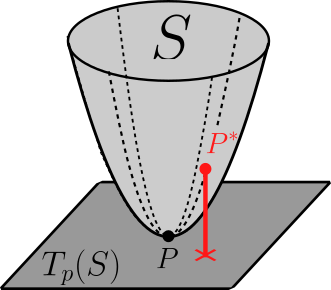
\includegraphics[scale=.5]{FOTOS/curvatura_dist.png}
\end{wrapfigure}

Consideramos un punto $P^*\in S$ infinitesimalmente próximo al punto $P$, de tal modo que las coordenadas de $P$ y $P^*$ son, respectivamente, $(u^1,u^2),(u^1+h^1,u^+h^2)$. Para medir la curvatura, estudiaremos cuánto se separa la superficie $S$ de $T_p(S)$.
$$
d(P^*,T_p(S))=(\mathbf{x}(u^p+h^p)-\mathbf{x}(u^p))\cdot \mathbf{n}
$$

Como $P$ y $P^*$ están infinitamente cerca, podemos expandir en serie de Taylor:
$$
\mathbf{x}(u^p+h^p)=\mathbf{x}(u^p)+\mathbf{x}_\alpha \cdot h^\alpha +\frac{1}{2}\mathbf{x}_{\alpha \beta }(u^p)\cdot h^\alpha h^\beta +\mathbf{R}_2
$$
Por lo que la distancia queda como:
\begin{equation*}
    \begin{split}
        d(P^*,T_p(S))&=\left ( \mathbf{x}_\alpha(u^p)\cdot h^\alpha +\frac{1}{2}\mathbf{x}_{\alpha \beta }(u^p)\cdot h^\alpha h^\beta +\ldots   \right )\cdot \mathbf{n}\\
        &=\frac{1}{2}\mathbf{x}_{\alpha \beta }\cdot \mathbf{n}h^\alpha h^\beta \qquad \text{porque }\mathbf{x}_\alpha \cdot \mathbf{n}=0
    \end{split}
\end{equation*}
Al producto escalar de la segunda derivada con el vector perpendicular a $T_p(S)$ lo llamaremos \emph{segunda forma fundamental}.
$$\boxed{b_{\alpha \beta }=\mathbf{x}_{\alpha \beta }\cdot \mathbf{n}}$$

Otra manera alternativa de expresar la segunda forma fundamental se obtiene derivando la expresión $\mathbf{x}_\alpha \cdot \mathbf{n}=0$:
$$
\mathbf{x}_{\alpha \beta }\cdot \mathbf{n}+\mathbf{x}_\alpha \mathbf{n}_\beta =0 \implies \boxed{b_{\alpha \beta }=-\mathbf{x}_\alpha \cdot \mathbf{n}_\beta }
$$

Para el determinante de esta matriz, utilizaremos la notación $b=\det{b_{\alpha \beta }}$. El nombre de segunda forma fundamental proviene de que la distancia $d(P^*,T_p(S))=1/2b_{\alpha \beta }h^\alpha h^\beta +\ldots $ es, a orden dominante, una forma cuadrática:
$$
Q(h^\alpha )=\frac{1}{2}b_{\alpha \beta }h^\alpha h^\beta 
$$

No obstante, al contrario que de la primera forma fundamental, esta \emph{no} tiene porqué ser definida positiva. 
\begin{mybox}
    \begin{center}
        \textbf{SEGUNDA FORMA FUNDAMENTAL}
    \end{center}
    $$
    b_{\alpha \beta }=\mathbf{x}_{\alpha \beta }\cdot \mathbf{n}=-\mathbf{x}_\alpha \cdot \mathbf{n}_\beta 
    $$
    \textbf{Propiedades:}
    \begin{enumerate}
        \item Si $b_{\alpha \beta }=0$ sobre una cierta carta local, la superficie en esa carta es un \textbf{plano}, y viceversa.
        \item $b_{\alpha \beta} $ son las componentes covariantes de un (pseudo-)tensor de segundo orden.
        \item La ley de transformación de $b$ es $\Bar{b}=D^2b$.
    \end{enumerate}
\end{mybox}
\begin{enumerate}
    \item[\fbox{1}] 
    \begin{proof}
            Suponemos que $b_{\alpha \beta }=0$, y sabemos que $||\mathbf{n}||=1 \leftrightarrow \mathbf{n}\cdot \mathbf{n}=1$. Derivando: $\mathbf{n}_\alpha \cdot \mathbf{n}+\mathbf{n} \cdot \mathbf{n}_\alpha\implies \mathbf{n}\cdot \mathbf{n}_\alpha =0 \iff \mathbf{n}_\alpha \in T_p(S)$. Esto significa que $\mathbf{n}_\alpha $ puede expresarse como combinación lineal de la base $\{ \mathbf{x}_1,\mathbf{x}_2 \} $. Por tanto:
            $$
            \left \{ \begin{array}{c}
                 b_{\alpha \beta }=0  \\
                 \mathbf{n}_\alpha \in T_p(S) 
            \end{array} \right . \implies \mathbf{x}_\alpha \cdot \mathbf{n}_\beta =0\iff \mathbf{n}\equiv \text{const.} 
            $$
            Entonces:
            $$
            (\mathbf{x}\cdot \mathbf{n})_\alpha =\cancelto{0}{\mathbf{n}\cdot \mathbf{x}_\alpha }+\cancelto{0}{\mathbf{n}_\alpha \cdot \mathbf{x}}
            $$
            Luego:
            $$
            \mathbf{x}\cdot \mathbf{n}\equiv \text{const.}\qquad \text{Ecuación de un plano.} 
            $$
    \end{proof}
    \item[\fbox{2}]
    \begin{proof}
        Si cambiamos de coordenadas $u^\alpha $ a $\Bar{u}^\beta $:
        \begin{equation*}
        \begin{split}
            \Bar{\mathbf{n}}=\frac{\Bar{\mathbf{x}}_1\wedge \Bar{\mathbf{x}}_2}{||\Bar{\mathbf{x}}_1\wedge \Bar{\mathbf{x}}_2||}\longrightarrow \Bar{b}_{\alpha \beta }=-\Bar{\mathbf{x}}_\alpha \cdot \Bar{\mathbf{n}}_\beta &=-\left ( \pdv{u^\mu }{\Bar{u}^\alpha } \mathbf{x}_\mu \right ) \cdot \left ( \pdv{u^\nu }{\Bar{u}^\beta } \mathbf{n}_\nu \right )\\
            &=- \pdv{u^\mu }{\Bar{u}^\alpha }\pdv{u^\nu }{\Bar{u}^\beta }\underbrace{\mathbf{x}_\mu\cdot \mathbf{n}_\nu}_{-b_{\mu \nu }}\\
            &=\pdv{u^\mu }{\Bar{u}^\alpha }\pdv{u^\nu }{\Bar{u}^\beta }b_{\mu \nu }
        \end{split}
        \end{equation*}
    \end{proof}
\end{enumerate}
\subsection{Clasificación de los puntos de una superficie}
Dada la superficie $S$, el plano tangente $T_p(S)$ y el punto $P^*$ de la superficie infinitesimalmente cerca de $P$, podemos clasificar las superficies en función de las diferentes separaciones del plano tangente.
\begin{itemize}
    \item \underline{PUNTO ELÍPTICO}: Si $b>0$, la superficie se comporta localmente como un paraboloide de revolución (o elíptico).
    $$
    Q(h^\alpha )=\frac{1}{2}b_{\alpha \beta }h^\alpha h^\beta 
    $$
    Además, si $b_{11}>0$, la superficie está orientada en el sentido de $\mathbf{n}$ (como el paraboloide elíptico, por ejemplo).\\
    Por el contrario, si $b_{11}<0$, la superficie está orientada en el sentido contrario a $\mathbf{n}$.

    \item \underline{PUNTO HIPERBÓLICO}: Si $b<0$, la superficie se comporta localmente como un paraboloide hiperbólico (punto de silla).
    \item \underline{PUNTO PARABÓLICO}: Si $b=0$ pero $b_{\alpha \beta }\neq 0$, la superficie se comporta localmente como un cilindro parabólico.
\end{itemize}

    \begin{wrapfigure}{r}{.3\textwidth}
    \centering
        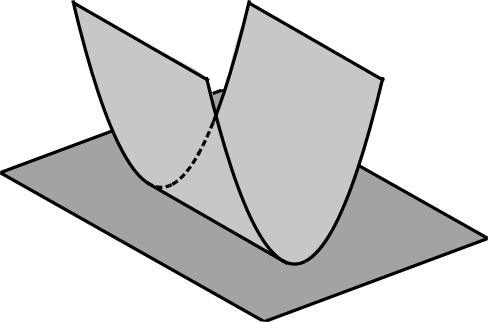
\includegraphics[scale=.3]{FOTOS/punto_parabolico.png}
        \caption*{Cilindro parabólico}
    \end{wrapfigure}
Si $b_{\alpha \beta}=0$ (es decir, la segunda forma fundamental se anula), entonces no podemos conocer la forma local de la superficie. En este caso, es necesario tomar el siguiente orden de aproximación en el desarrollo en serie de Taylor. A este tipo de puntos se les conoce como \underline{PUNTOS PLANARES}.\\

\WFclear
\begin{mybox}
\begin{wrapfigure}{r}{.36\textwidth}
        \centering
        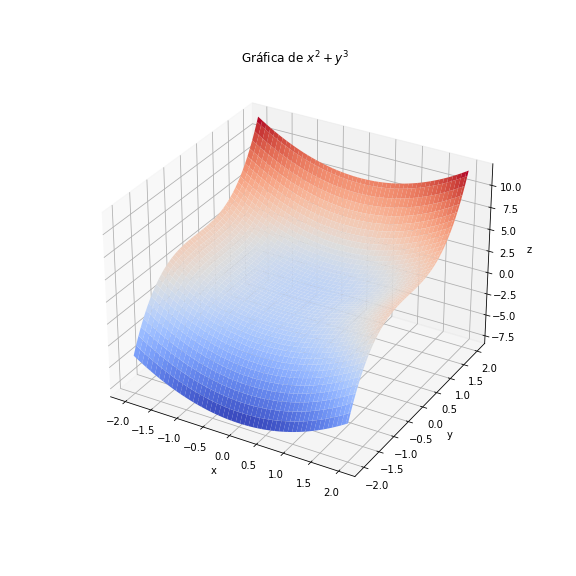
\includegraphics[scale=.3]{FOTOS/ejemplo3_A.png}
        \caption*{Gráfica de $f(x,y)=x^2+y^3$}
    \end{wrapfigure}
 \underline{Ejemplo A:} $\mathbf{x}(u^1,u^2)=(u^1,u^2,(u^1)^2+(u^2)^3)$
    
    $$\mathbf{x}_1=(1,0,2u^1),\ \mathbf{x}_2=(0,1,3(u^2)^2)$$
    $$
    \mathbf{n}=\frac{\mathbf{x}_1\wedge \mathbf{x}_2}{||\mathbf{x}_1\wedge \mathbf{x}_2||}=\frac{(-2u^1,-3(u^2)^2,1)}{\sqrt{1+(u^1)^2+9(u^2)^4}}
    $$
    $$
    b_{\alpha \beta }=\mathbf{x}_{\alpha \beta }\cdot \mathbf{n}
    $$
    $\implies 
    \left \{ \begin{array}{ccccc}
         \mathbf{x}_{11}&=&(0,0,2)&&  \\
         \mathbf{x}_{12}&=&(0,0,0)&=&\mathbf{x}_{21}\\
         \mathbf{x}_{22}&=&(0,0,6u^2)&&
    \end{array} \right .
    $\\
    $
    \implies \left \{ \begin{array}{ccccc}
         b_{11}&=&\frac{2}{\sqrt{1+(u^1)^2+9(u^2)^4}}&&  \\
         b_{12}&=&0&=&b_{21}\\
         b_{22}&=&\frac{6u^2}{\sqrt{1+(u^1)^2+9(u^2)^4}}&&\\
    \end{array} \right .\\
    $\WFclear$  \text{Es decir: \quad \parbox{8cm}{$b>0$ si $u^2>0$: puntos elípticos\\
                                                                 $b<0$ si $u^2<0$: puntos hiperbólicos\\
                                                                 $b=0$ si $u^2=0$: puntos parabólicos}}$
\end{mybox}

\section{Curvaturas principales, media y gaussiana}
\begin{wrapfigure}{l}{.35\textwidth}
    \centering
    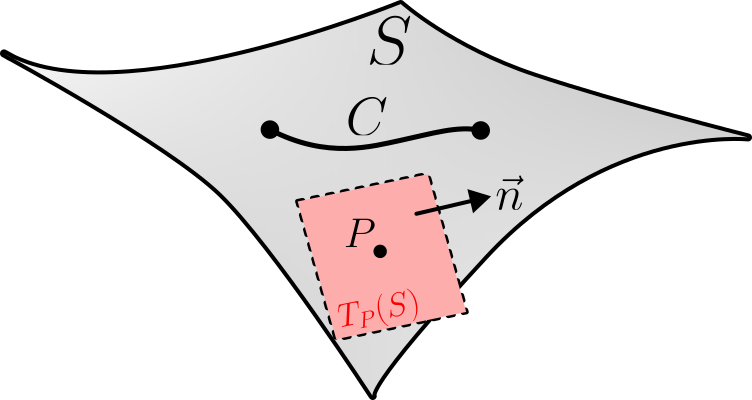
\includegraphics[scale=.26]{FOTOS/cpmg_1.png}
    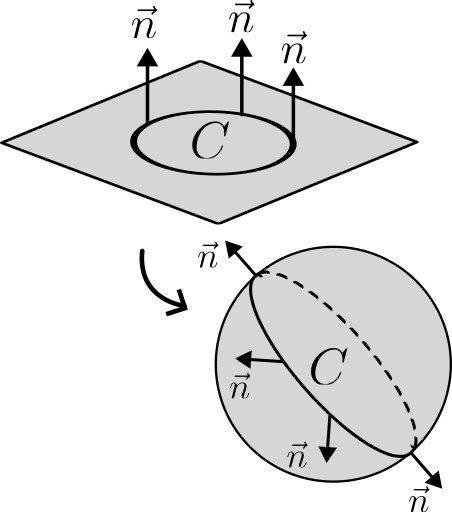
\includegraphics[scale=.35]{FOTOS/cpmg_2.png}
\end{wrapfigure}
La curvatura de una curva contenida dentro de una superficie dependerá de la propia curva y de la curvatura de la superficie. Como ejemplo, podemos pensar en una circunferencia contenida en un plano, o la misma circunferencia entendida como el ecuador de una esfera. \\

La contribución a la curvatura de la curva que proviene de la superficie se debe a cómo varía el vector normal sobre la superficie y, en concreto, del ángulo que forman entre $\mathbf{n}$ y $\mathbf{k}$, con $\mathbf{k}=k\cdot \mathbf{p}$, donde $\mathbf{p}$ es el vector normal principal de la curva. Para ver esto, descompondremos $\mathbf{k}$, el vector de curvatura, en una componente \emph{normal} (o paralela a $\mathbf{n}$); y en otra no paralela.\\
$$
\mathbf{k}=\mathbf{k}_n+\mathbf{k}_g \qquad \qquad \mathbf{k}_n\cdot \mathbf{n}=0 \ (\mathbf{k}_n\parallel \mathbf{n})
$$
$\mathbf{k}_g$ será entonces el vector de curvatura \emph{geodésica} (debida al tipo de curva). \\

Sea $S$ una superficie parametrizada, y $C$ una determinada curva en $S$, parametrizada en términos de la longitud de arco ($||\dot{\mathbf{x}}(S)||=1)$.
$$
\mathbf{k}_n=k_n\cdot \mathbf{n} \qquad \text{y} \qquad k_n=\mathbf{k}\cdot \mathbf{n}
$$
Como $\mathbf{k}$, para una curva en parámetro natural, es $\mathbf{k}=\dot{\mathbf{t}}=\ddot{\mathbf{x}}$; al aplicar la regla de la cadena queda:
\begin{gather*}
    \ddot{\mathbf{x}}=\pdv{\mathbf{x}}{u^\alpha }\dot{u}^\alpha =\mathbf{x}_{\alpha \beta }\dot{u}^\alpha \dot{u}^\beta +\mathbf{x}_\alpha \ddot{u}^\alpha \\
    \implies k_n=\ddot{\mathbf{x}}\cdot \mathbf{n}=(\mathbf{x}_{\alpha \beta }\dot{u}^\alpha \dot{u}^\beta +\mathbf{x}_\alpha \ddot{u}^\alpha)\cdot \mathbf{n}=b_{\alpha \beta }\dot{u}^\alpha \dot{u}^\beta 
\end{gather*}
En el caso de encontrarnos en una parametrización arbitraria:
$$
\dot{u}^\alpha =\dv{u^\alpha }{S}=\dv{u^\alpha }{t}\cdot \dv{t}{S}=(u^\alpha )'\cdot \frac{1}{||\mathbf{x}'(t)||}
$$
De esta forma, 
$$
k_n=\frac{1}{||\mathbf{x}'(t)||^2}b_{\alpha \beta }(u^\alpha )'(u^\beta)'=\boxed{\frac{b_{\alpha \beta }(u^\alpha )'(u^\beta )'}{g_{\mu \nu }(u^\mu )'(u^\nu )'}=k_n}
$$

La \emph{curvatura normal} es el cociente entre la segunda y la primera forma fundamental, evaluadas sobre la curva (conocidas $u^\alpha =u^\alpha (t)$). La curvatura normal es, en realidad, el ángulo entre $\mathbf{n}$ y el vector de curvatura $\mathbf{k}$ (o $\mathbf{p}$). \\
\newpage
\begin{wrapfigure}{r}{.35\textwidth}
    \centering
    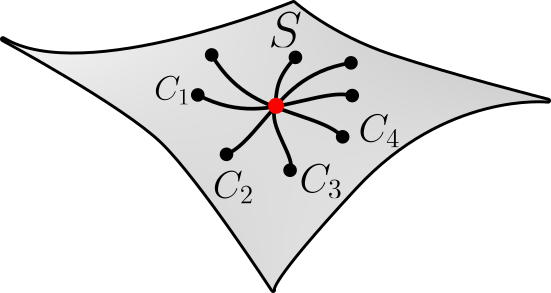
\includegraphics[scale=.37]{FOTOS/curva_normal.png}
\end{wrapfigure}
La curvatura de cada curva $C_i$ (las cuales pasan todas por el mismo punto), serán distintas, como aparece en la imagen. Para ello, definiremos las curvaturas normales principales de la superficie $S$ en el punto $P$.\\

\subsection{Curvaturas normales principales (de $S$ en $P$)}
Se definen como los valores mayor y menor de la curvatura normal para todas las curvas contenidas en esa superficie $S$ y que pasan por el punto $P$.\\

Por comodidad, introducimos la siguiente notación:
\paragraph{Notación:} $(u^\alpha )'=\dv{u^\alpha (t)}{t}=\ell ^\alpha \implies k_n=\frac{b_{\alpha \beta }\ell ^\alpha \ell ^\beta }{g_{\mu \nu }\ell ^\mu \ell ^\nu }=\frac{A}{B}$, con $A=b_{\alpha \beta }\ell ^\alpha \ell ^\beta $ y $B=g_{\mu \nu} \ell ^\mu \ell ^\nu $.\\

Para hallar los valores de $k_n$ máximos y mínimos, derivamos la curvatura normal e imponemos que sea nula.
$$
\pdv{k_n}{\ell ^\alpha }=0=\frac{B\pdv*{A}{\ell ^\alpha }-A\pdv*{B}{\ell ^\alpha }}{B^2}
$$
Si multiplicamos por $B$ y usamos que $k_n=A/B$, entonces la expresión anterior puede escribirse como:
$$
\pdv{A}{\ell^\alpha }-k_n\pdv{B}{\ell ^\alpha }=0
$$
y, junto con las expresiones explícitas de $A$ y $B$, llegamos a que:
$$
(b_{\alpha \beta }l^\beta +b_{\beta \alpha }\ell ^\beta )-k_n(g_{\alpha \beta }\ell ^\beta +g_{\beta \alpha }\ell ^\beta )=0
$$
Como $g_{\alpha \beta }$ y $b_{\alpha \beta}$ son simétricas en $\alpha $ y $\beta $, la expresión se simplifica:
\begin{gather*}
    (b_{\alpha \beta }-k_ng_{\alpha \beta})\ell ^\beta =0 \quad (\alpha ,\beta =1,2)\\
    \left .\begin{array}{cc}
         \alpha =1:&(b_{11}-k_ng_{11})\ell ^1+(b_{12}-k_ng_{12})\ell^2=0  \\
         \alpha =2:&(b_{21}-k_ng_{21})\ell ^1+(b_{22}-k_ng_{22})\ell^2=0
    \end{array} \right \} 
\end{gather*}
que es un sistema homogéneo con $(\ell^1,\ell^2)\neq (0,0)$. Por tanto, para las soluciones no triviales, el determinante de la matriz de coeficientes debe de ser nulo.
$$
\left | \begin{array}{cc}
     b_{11}-k_ng_{11}&b_{12}-k_ng_{12}  \\
     b_{21}-k_ng_{21}&b_{22}-k_ng_{22} 
\end{array} \right |=0
$$
Esta condición proporciona una ecuación con dos soluciones para $k_n$. Estas dos soluciones, que etiquetaremos $k_1$ y $k_2$ ($k_1\ge k_2$), se conocen como las \emph{curvaturas normales principales} de la superficie $S$ en el punto $P$.\\

Para calcular las curvaturas normales $k_1$ y $k_2$, introduciremos el \emph{operador de Weingarten}, que es la segunda forma fundamental con un índice covariante y otro contravariante.
$$
b^\mu {}_\nu \equiv \text{operador de Weingarten.}
$$
De la ecuación $(b_{\alpha \beta }-k_ng_{\alpha \beta})\ell ^\beta =0$, tenemos que 
\begin{gather*}
    g^{\alpha \mu}(b_{\alpha \beta }-k_ng_{\alpha \beta})\ell ^\beta =0\\
    \implies (b^\mu {}_\beta -k_n \delta ^\mu {}_\beta )\ell ^\beta =0\\
    \implies \left | \begin{array}{cc}
        b^1{}_1-k_n &b^1{}_2  \\
         b^2{}_1&b^2{}_2-k_n 
    \end{array} \right |=0
\end{gather*}
(que es una ecuación de autovalores para el operador de Weingarten). Desarrollando: 
$$
k_n^2-(b^1{}_1+b^2{}_2)k_n+(b^1{}_1b^2{}_2-b^2{}_1b^1{}_2)=0
$$
Si usamos que $b^1{}_1+b^2{}_2=b^\alpha {}_\alpha $ y que $\det(b^\mu {}_\nu )=\det(g^{\mu \alpha }b_{\alpha \nu})=\det(g^{\mu \nu })\det(b_{\alpha \nu})=b/g$, obtenemos la siguiente expresión:
$$
\boxed{k_n^2-b^\alpha {}_\alpha k_n+\frac{b}{g}=0}
$$

Las ecuaciones algebraicas de segundo grado pueden escribirse en términos de sus soluciones.
\begin{gather*}
    (k_n-k_1)(k_n-k_2)=0\\
    =k_n^2-(k_1+k_2)k_n+k_1k_2=0\\
    \implies k_1k_2=\frac{b}{g} \qquad k_1+k_2=b^\alpha {}_\alpha 
\end{gather*}

Y, finalmente, usando estas relaciones, podemos definir dos curvaturas para la superficie:
\begin{mybox}
    \begin{center}
        \textbf{CURVATURA MEDIA}
    \end{center}
    $$
    H\equiv \frac{1}{2}(k_1+k_2)=\frac{1}{2}b^\alpha {}_\alpha 
    $$
    Esta curvatura depende tanto de la primera forma fundamental como de la segunda forma fundamental.
    \begin{center}
        \textbf{CURVATURA GAUSSIANA}
    \end{center}
    $$
    K\equiv k_1\cdot k_2=\frac{b}{g}
    $$
    Al contrario de la curvatura media, esta curvatura \textbf{sólo depende de la primera forma fundamental}, al poder escribirse el determinante $b$ en términos de $g$.
\end{mybox}

A partir de esta definición, se dice que una superficie es \emph{minimal} si $H=0$ en todos sus puntos (el nombre se debe a que este tipo de superficies pueden probarse que tienen área mínima. Este es el caso del plano). Veamos cómo se transforman estas dos cantidades $H$ y $K$ bajo cambios de coordenadas. 

Como $b_{\alpha \beta }$ es un pseudo-tensor y $g_{\alpha \beta }$ es un tensor, $k_n$ sólo cambiará de signo si cambia el sentido de $\mathbf{n}$. Por tanto, el producto de $k_1k_2=K$ será \emph{invariante} bajo cambios de coordenadas. En consecuencia, la curvatura gaussiana $K$ es un \emph{escalar}. (también puede verse este hecho con las leyes de transformación tensoriales).
\section{Fórmulas de Weingarten y de Gauss. Símbolos de Christoffel}
Como hemos visto en el capítulo 1, el sistema de Frenet se adapta a la geometría de la curva que estudiamos (se desplaza con el parámetro $t$). La evolución de este sistema da lugar a la noción de curvaturas de una curva en $\mathbb{R}^n$. \\

En el caso de las superficies, escribiremos $\{ \mathbf{x}_{\alpha \beta },\mathbf{n}_\beta  \}$ en términos de $\{ \mathbf{x}_\alpha ,\mathbf{n} \}$, con $\alpha ,\beta =1,2$. Derivaremos los vectores $\{ \mathbf{x}_1,\mathbf{x}_2,\mathbf{n} \}$ con respecto a las coordenadas curvilíneas locales, 
$$
\mathbf{x}_{\alpha \beta }=\partial_\beta \mathbf{x}_\alpha =\Gamma_{\alpha \beta }{}^\gamma \mathbf{x}_\gamma +a_{\alpha \beta }\mathbf{n}
$$
$$
\mathbf{n}_\beta =\partial_\beta \mathbf{n}=c_\beta {}^\gamma \mathbf{x}_\gamma +d_\beta \mathbf{n}
$$
donde $\Gamma_{\alpha \beta}{}^\gamma ,a_{\alpha \beta} ,c_\beta ,d_\beta $ son los coeficientes. Analizamos primero la segunda ecuación: como $||\mathbf{n}||^2=\mathbf{n}\cdot \mathbf{n}=1,\ \mathbf{n}_\beta \cdot \mathbf{n}=0 \implies d_\beta =0$. 

Si usamos la base dual,
\begin{gather*}
    \mathbf{x}^\gamma \cdot \mathbf{n}_\beta =g^{\gamma \rho} \mathbf{x}_\rho \cdot \mathbf{n}_\beta=-g^{\gamma \rho} b_{\rho \beta }=-b^\gamma {}_\beta \\
    \implies \mathbf{x}^\gamma \cdot \mathbf{n}_\beta =c_\beta {}^\gamma =-b_\beta {}^\gamma 
\end{gather*}

De la primera ecuación, $\mathbf{n}\cdot \mathbf{x}_{\alpha \beta}=a_{\alpha \beta }$. Por definición, $b_{\alpha \beta }=\mathbf{n}\cdot \mathbf{x}_{\alpha \beta }$, de modo que $\mathbf{n}\cdot \mathbf{x}_{\alpha \beta }=a_{\alpha \beta }=b_{\alpha \beta }$. 

Si utilizamos la base dual, $\mathbf{x}^\gamma \cdot \mathbf{x}_{\alpha \beta }=\boxed{\Gamma _{\alpha \beta }{}^\gamma} $. Estas cantidades se conocen como los \emph{símbolos de Christoffel de segunda especie} (no son tensores). Los símbolos de Christoffel \emph{de primera especie} son:
$$
\Gamma _{\alpha \beta \gamma }=\mathbf{x}_\gamma \cdot \mathbf{x}_{\alpha \beta }=g_{\mu \gamma }\Gamma ^\mu{}_{\alpha \beta }
$$

La notación usada en la literatura matemática es $\Gamma _{\alpha \beta }{}^\gamma $. En física--y, en concreto, en Relatividad General-- usamos la notación $\Gamma ^\gamma {}_{\alpha \beta }$. \\

Con esta definición, las ecuaciones anteriores pueden escribirse como:
\begin{align}
    \mathbf{x}_{\alpha \beta }&=\Gamma _{\alpha \beta }{}^\gamma \mathbf{x}_\gamma +b_{\alpha \beta }\mathbf{n} &&\text{: Ecuación de Gauss} \tag*{[G]} \label{gauss}\\
    \mathbf{n}_\beta &=-b_\beta {}^\gamma \cdot \mathbf{x}_\gamma &&\text{: Ecuación de Weingarten} \tag*{[W]} \label{weingarten}
\end{align}
$$
b_{\alpha \beta }=\mathbf{n}\cdot \mathbf{x}_{\alpha \beta } \qquad \qquad \Gamma _{\alpha \beta }{}^\gamma =\mathbf{x}^\gamma \cdot \mathbf{x}_{\alpha \beta }
$$
\section{Propiedades de los símbolos de Christoffel}
\subsection{Simetrías}
Del \emph{teorema de Schwarz} \footnote{Básicamente, si $f(x,y)$ es continua en su dominio abierto $D$ y es de clase $C^2$, entonces $f_{xy}=f_{yx}$.}, $\mathbf{x}_{\alpha \beta }=\mathbf{x}_{\beta \alpha }$, con $\alpha ,\beta =1,2$, luego los símbolos de Christoffel, $\Gamma _{\alpha \beta }{}^\gamma =\mathbf{x}^\gamma \cdot \mathbf{x}_{\alpha \beta }$ son simétricos bajo el intercambio de $\alpha $ y $\beta $.
$$
\Gamma _{\alpha \beta }{}^\gamma =\Gamma _{\beta \alpha  }{}^\gamma 
$$
Esto significa que, de los $2\times 2\times 2=8$ símbolos posibles en un superficie, sólo 6 de ellos son independientes (en dimensión $n$, serían $n^2(n+1)/2$).\\

Gracias a esta simetría, es posible obtener los símbolos de Christoffel en términos de derivadas de la primera forma fundamental. Esta expresión será la definición más común para estos símbolos. \\

Habíamos definido la primera forma fundamental como:
$$
g_{\alpha \lambda }=\mathbf{x}_\alpha \cdot \mathbf{x}_\lambda ,\ \text{con }\alpha ,\lambda=1,2.
$$
Si derivamos con respecto a $u^\beta $:
\begin{equation} \label{[*]}\tag*{[*]}
    \begin{split}
        \pdv{g_{\alpha \lambda  }}{u^\beta }&=\mathbf{x}_{\alpha \beta }\cdot \mathbf{x}_\lambda +\mathbf{x}_\alpha \cdot \mathbf{x}_{\lambda \beta }\\
        &=\Gamma_{\alpha \beta \lambda }+\Gamma _{\lambda \beta \alpha }
    \end{split}
\end{equation}
Si ahora rotamos los índices cíclicamente: $\alpha \rightarrow \beta \rightarrow \lambda \rightarrow \alpha $
\begin{equation} \label{[**]}
    \pdv{g_{\beta \alpha }}{u^\lambda }=\Gamma _{\beta \lambda }+\Gamma _{\alpha \lambda \beta } \tag*{[**]}
\end{equation}
\begin{equation}\label{[***]}
    \pdv{g_{\lambda \beta }}{u^\alpha }=\Gamma _{\lambda \alpha \beta }+\Gamma _{\beta \alpha \lambda }\tag*{[***]}
\end{equation}
Si ahora calculamos \ref{[*]}+\ref{[***]}-\ref{[**]}:
$$
\pdv{g_{\alpha \lambda  }}{u^\beta }+\pdv{g_{\lambda \beta }}{u^\alpha }-\pdv{g_{\beta \alpha }}{u^\lambda }=2\Gamma _{\alpha \beta \lambda }
$$
Por lo que, finalmente, podemos escribir:
$$
\boxed{\Gamma _{\alpha \beta \lambda }=\frac{1}{2}\left ( \pdv{g_{\alpha \lambda  }}{u^\beta }+\pdv{g_{\lambda \beta }}{u^\alpha }-\pdv{g_{\beta \alpha }}{u^\lambda } \right )}
$$
que es la definición para los símbolos de Christoffel de primera especie. \\

Para los símbolos de Christoffel de segunda especie, usamos la primera forma fundamental en notación contravariante.
\begin{mybox}
    \begin{center}
        \textbf{DEFINICIÓN DE SÍMBOLOS DE CHRISTOFFEL}
    \end{center}
    De primera especie:
    $$
    \Gamma _{\alpha \beta \lambda }=\frac{1}{2}\left ( \pdv{g_{\alpha \lambda  }}{u^\beta }+\pdv{g_{\lambda \beta }}{u^\alpha }-\pdv{g_{\beta \alpha }}{u^\lambda } \right )
    $$
    De segunda especie:
    $$
    \Gamma _{\alpha \beta }{}^\mu =g^{\mu \lambda }\Gamma _{\alpha \beta \lambda }=\frac{1}{2}g^{\mu \lambda }\left ( \pdv{g_{\alpha \lambda  }}{u^\beta }+\pdv{g_{\lambda \beta }}{u^\alpha }-\pdv{g_{\beta \alpha }}{u^\lambda } \right )
    $$
    \noindent\rule{\textwidth}{0.5pt}
    \underline{Ejemplo B:}
    \begin{enumerate}
        \item[(i)] Símbolos de Christoffel para coordenadas ortogonales sobre una superficie $S$.
        $$
        g_{\alpha \beta }=g_{\alpha \beta }(u^1,u^2)=\left ( \begin{array}{cc}
             g_{11}&  \\
             & g_{22}
        \end{array} \right )\rightarrow g^{\alpha \beta }=\left ( \begin{array}{cc}
             1/g_{11}&  \\
             & 1/g_{22}
        \end{array} \right )
        $$
        Los símbolos de Christoffel son $\Gamma _{11}{}^1=g^{1\lambda }\Gamma _{11\lambda }$.
        \begin{equation*}
            \begin{split}
                \Gamma _{11}{}^1&=g^{11}\Gamma_{111}+\cancel{g^{12}\Gamma _{112}}=\frac{1}{2g_{11}}\left ( \pdv{g_{11}}{u^1}+\cancel{\pdv{g_{11}}{u^1}}-\cancel{\pdv{g_{11}}{u^1}} \right )\\
                &=\frac{1}{2g_{11}}\pdv{g_{11}}{u^1}(u^1,u^2)
            \end{split}
        \end{equation*}
        \begin{gather*}
            \Gamma _{22}{}^1=-\frac{1}{2g_{11}}\pdv{g_{22}}{u^1} ,\quad \Gamma_{11}{}^2=-\frac{1}{2g_{11}}\pdv{g_{11}}{u^2} ,\quad \Gamma_{22}{}^2=\frac{1}{2g_{22}}\pdv{g_{22}}{u^2} \\
            \Gamma_{12}{}^1=\Gamma_{21}{}^1=\frac{1}{2g_{11}}\pdv{g_{11}}{u^2},\quad \Gamma_{12}{}^2=\Gamma_{21}{}^2=\frac{1}{2g_{22}}\pdv{g_{22}}{u^1}
        \end{gather*}

        \item[(ii)] Símbolos de Christoffel para el plano en coordenadas polares:\\
        $
        \mathbf{x}(u^1,u^2)=(u^1\cos u^2,u^1 \sin u^2,0) \quad (r,\theta)
        $
        $$
        g_{\alpha \beta }=\left ( \begin{array}{cc}
            1 &  \\
             & (u^1)^2
        \end{array} \right )=\left ( \begin{array}{cc}
             1&  \\
             &r^2 
        \end{array} \right )
        $$
        $$
        \Gamma_{22}{}^1=\Gamma_{rr}{}^\theta =-r ,\quad \Gamma_{12}{}^2=\Gamma_{21}{}^2=\Gamma_{r\theta}{}^\theta =\Gamma_{\theta r}{}^\theta =1/r
        $$
    \end{enumerate}
\end{mybox}
Una relación útil de los símbolos de Christoffel es la de la contracción de símbolos:
$$
\Gamma_{\alpha \beta }{}^\alpha =\frac{1}{2}g^{\alpha \lambda}\left ( \pdv{g_{\alpha \lambda}}{u^\beta }+ \cancel{\pdv{g_{\beta  \lambda}}{u^\alpha }}-\cancel{\pdv{g_{\alpha \beta}}{u^\lambda  }}\right )=\frac{1}{2}g^{\alpha \lambda}\pdv{g_{\alpha \lambda }}{u^\beta }
$$
Otra relación útil es la siguiente:
$$
\pdv{g}{u^\beta }=\pdv{}{u^\beta }\left (g_{11}g_{22}-(g_{12})^2\right )=\partial_\beta g_{11} g_{22}+g_{11}\partial_\beta g_{22}-2g_{12}\partial_\beta g_{12}
$$
Además: $g_{\alpha \beta }=\left ( \begin{array}{cc}
     g_{11}&g_{12}  \\
     g_{21}& g_{22}
\end{array} \right )\Rightarrow  g^{11}=g_{22}/g,\ g^{22}=g_{11}/g$, $g^{12}=g^{21}=-g_{12}/g$, luego:
$$
\partial_\beta g=gg^{11}\partial_\beta g_{11}+gg^{22}\partial_\beta g_{22}+2gg^{12}\partial_\beta g_{12}=gg^{\alpha \lambda} \pdv{g_{\alpha \lambda }}{u^\beta }
$$
Combinando los dos resultados:
$$
\boxed{\Gamma_{\alpha \beta }{}^\alpha =\frac{1}{2g}\pdv{g}{u^\beta }=\pdv{}{u^\beta }[\log \sqrt{g}]}
$$
\subsection{Ley de transformación de los símbolos de Christoffel}
$(U,\mathbf{x}(u^\alpha )\longrightarrow (\Bar{U},\Bar{\mathbf{x}}(\Bar{u}^\alpha )$: Al cambiar de parametrización:
$$
\Bar{\mathbf{x}}_\alpha =\pdv{u^\gamma }{\Bar{u}^\alpha }\mathbf{x}_\gamma  \quad , \quad \Bar{\mathbf{x}}^\lambda =\pdv{\bar{u}^\lambda }{u^\sigma }\mathbf{x}^\sigma 
$$
La segunda derivada cumple:
$$
\Bar{\mathbf{x}}_{\alpha \beta }=\pdv{}{\Bar{u}^\beta }\Bar{\mathbf{x}}_\alpha =\pdv{u^\gamma }{\Bar{u}^\alpha }\pdv{u^\mu }{\Bar{u}^\beta }\mathbf{x}_{\gamma \mu }+\pdv{u^\gamma }{\Bar{u}^\alpha }{\Bar{u}^\beta }\cdot \mathbf{x}_\gamma 
$$
Es decir, los símbolos de Christoffel (de segunda especie) en las nuevas coordenadas (carta $(\Bar{U},\Bar{\mathbf{x}}(\Bar{u}^\alpha ))$) son:
\begin{equation*}
    \begin{split}
        \Bar{\Gamma }_{\alpha \beta }{}^\lambda =\Bar{\mathbf{x}}_{\alpha \beta }\cdot \Bar{\mathbf{x}}^\lambda &=\color{red}\pdv{u^\gamma }{\Bar{u}^\alpha }\pdv{u^\mu }{\Bar{u}^\beta }\pdv{\Bar{u}^\lambda }{u^\sigma }\overbrace{\mathbf{x}_{\gamma \mu }\cdot \mathbf{x}^\sigma }^{\Gamma_{\gamma \mu }{}^\sigma }\color{blue} +\pdv{u^\gamma }{\Bar{u}^\alpha }{\Bar{u}^\beta }\pdv{\Bar{u}^\lambda }{u^\sigma }\underbrace{\mathbf{x}_\gamma \cdot \mathbf{x}^\sigma }_{\delta_\gamma {}^\sigma }\\
        &=\color{red}{\pdv{u^\gamma }{\Bar{u}^\alpha }\pdv{u^\mu }{\Bar{u}^\beta }\pdv{\Bar{u}^\lambda }{u^\sigma }\Gamma_{\gamma \mu }{}^\sigma }\color{blue} +\pdv{u^\gamma }{\Bar{u}^\alpha }{\Bar{u}^\beta }\pdv{\Bar{u}^\lambda }{u^\sigma }
    \end{split}
\end{equation*}
El término en rojo corresponde a la ley de transformación tensorial habitual. El término azul 'estropea' este carácter tensorial de los símbolos de Christoffel (salvo reparametrizaciones lineales).
\section{Tensor de curvatura de Riemann}
Ahora deduciremos las \emph{ecuaciones de Mainardi-Codazzi}. Como hemos visto, a través de la superficie parametrizada podemos deducir información acerca de la curvatura de ésta:
$$
\mathbf{x}(u^1,u^2)\longrightarrow \mathbf{x}_\alpha =\partial _\alpha \mathbf{x}\longrightarrow g_{\alpha \beta }=\mathbf{x}_\alpha \cdot \mathbf{x}_\beta \longrightarrow \mathbf{n}\longrightarrow b_{\alpha \beta }\longrightarrow g,b,H,K\longrightarrow \Gamma _{\alpha \beta }{}^\gamma  
$$

Las ecuaciones de Mainardi-Codazzi establecen, fundamentalmente, que $\mathbf{x}_{\alpha \beta \gamma}=\mathbf{x}_{\alpha \gamma \beta }$, que es la condición de integrabilidad. Esto hace que la superficie no tenga ninguna obstrucción o patología, y existe una independencia sobre el camino que tomamos integrando entre dos puntos infinitesimalmente próximos. \\

Si derivamos la fórmula de Gauss, \ref{gauss}:
\begin{gather*}
    \mathbf{x}_{\alpha \beta }=\Gamma _{\alpha \beta }{}^\gamma \mathbf{x}_\gamma +b_{\alpha \beta }\mathbf{n}\implies \mathbf{x}_{\alpha \beta \gamma }=\pdv{}{u^\gamma }\mathbf{x}_{\alpha \beta }\\
    \pdv{}{u^\gamma }\mathbf{x}_{\alpha \beta }=\partial_\gamma \Gamma_{\alpha \beta}{}^\sigma \cdot \mathbf{x}_\sigma +\Gamma_{\alpha \beta}{}^\sigma \cdot \mathbf{x}_{\sigma \gamma }+\partial_\gamma b_{\alpha \beta }\cdot \mathbf{n}+b_{\alpha \beta }\cdot \mathbf{n}_\gamma
\end{gather*}
Y si ahora usamos la fórmula de Weingarten, \ref{weingarten}: $\mathbf{n}_\gamma =-b_\gamma {}^\sigma  \cdot \mathbf{x}_\sigma $, y la de Gauss:
\begin{equation*}
    \begin{split}
        \mathbf{x}_{\alpha \beta \gamma }&=\partial_\gamma \Gamma _{\alpha \beta }{}^\sigma \mathbf{x}_\sigma +\Gamma _{\alpha \beta }{}^\sigma \left ( \Gamma _{\sigma \gamma }{}^\rho \mathbf{x}_\rho +b_{\sigma \gamma }\cdot \mathbf{n} \right )+\partial_\gamma b_{\alpha \beta }\cdot \mathbf{n}-b_{\alpha \beta }b_\gamma {}^\sigma \mathbf{x}_\sigma \\
        \mathbf{x}_{\alpha \beta \gamma  }&=\left ( \partial_\gamma \Gamma _{\alpha \beta }{}^\sigma+ \Gamma _{\sigma \gamma }{}^\rho \Gamma _{\rho \gamma }{}^\sigma -b_{\alpha \beta} b_\gamma {}^\sigma \right )\cdot \mathbf{x}_\sigma +\left ( \Gamma _{\alpha \beta } {}^\sigma b_{\sigma \gamma }+\partial_\gamma b_{\alpha \beta } \right )  \cdot \mathbf{n}
    \end{split}
\end{equation*}
Como $\{ \mathbf{x}_\alpha ,\mathbf{n} \}$ son vectores linealmente independientes, al imponer la condición de $\mathbf{x}_{\alpha \beta \gamma }=\mathbf{x}_{\alpha \gamma \beta }$, los términos que vayan con cada vector deben ser idénticamente iguales, obteniéndose dos conjuntos de ecuaciones, que son las ecuaciones de Mainardi-Codazzi.
\begin{gather*}
    \pdv{\Gamma_{\alpha \beta }{}^\sigma }{u^\gamma }-\pdv{\Gamma _{\alpha \gamma }{}^\sigma }{u^\beta }+\Gamma _{\alpha \beta} {}^\rho\Gamma _{\rho \gamma }{}^\sigma -\Gamma _{\alpha \gamma }{}^\rho \Gamma _{\rho \beta }{}^\sigma =b_{\alpha \beta }b_\gamma {}^\sigma -b_{\alpha \gamma }b_\beta {}^\sigma \\
    \Gamma _{\alpha \beta }{}^\sigma b_{\sigma \gamma }-\Gamma _{\alpha \gamma }{}^\sigma b_{\sigma \beta }+\pdv{b_{\alpha \beta }}{u^\gamma }-\pdv{b_{\alpha \gamma }}{u^\beta }=0
\end{gather*}
\subsection{Tensor de curvatura de Riemann}
Analizando la primera ecuación de M-C, el lado derecho es un producto de segundas formas fundamentales. La segunda forma fundamental, $b_{\alpha \beta }=\mathbf{x}_{\alpha \beta }\cdot \mathbf{n}$, es un pseudo-tensor. El producto da lugar, por tanto, a algo que se comporta de forma \emph{tensorial}. En este caso, esto hace que sea un tensor de cuarto orden, tres veces covariante y una vez contravariante. \\

Por definición, el lado izquierdo de la primera ecuación se conoce como el \emph{tensor de curvatura de Riemann}.
$$
\boxed{R^\sigma {}_{\alpha \gamma \beta }\equiv \pdv{\Gamma_{\alpha \beta }{}^\sigma }{u^\gamma }-\pdv{\Gamma _{\alpha \gamma }{}^\sigma }{u^\beta }+\Gamma _{\alpha \beta} {}^\rho\Gamma _{\rho \gamma }{}^\sigma -\Gamma _{\alpha \gamma }{}^\rho \Gamma _{\rho \beta }{}^\sigma}
$$
Para presentar las simetrías del tensor de Riemann, trabajaremos con su versión cuatro veces covariante.
$$
R_{\mu \alpha \gamma \beta }=g_{\mu \sigma }R^\sigma {}_{\alpha \gamma \beta }=b_{\alpha \beta }b_{\gamma \mu} -b_{\alpha \gamma }b_{\beta \mu}
$$
Este tensor cumple las siguientes propiedades:
\begin{itemize}
    \item $R_{\mu \alpha \ \gamma \beta }= R_{ \gamma \beta \ \mu \alpha}$ (simetría por pares de índices)
    \item $R_{\mu \alpha  \gamma \beta }=-R_{\alpha  \mu  \gamma \beta }$ (antisimetría en los dos primeros índices)
    \item $R_{\mu \alpha  \gamma \beta }=-R_{\mu \alpha   \beta \gamma}$ (antisimetría en los dos últimos índices)
    \item $R_{\mu \alpha  \gamma \beta }+R_{\mu  \beta  \alpha  \gamma}+R_{\mu   \gamma \beta \alpha}=0$ (propiedad cíclica)
\end{itemize}

La construcción $R^\sigma {}_{\alpha \gamma \beta }$ es general, válida en dimensión $n$. Sus simetrías nos permiten reducir el número de componentes independientes a $n^2(n^2-1)/12$. En nuestro caso, $n=2$, una componente independiente. Las propiedades vistas anteriormente permiten reducir las componentes independientes de $n^4(n^2-1)/12$ a $n^2(n^2-1)/12$.
\section{Teorema egregio de Gauss}
Dada la superficie $\mathbf{x}(u^1.u^2)$, podemos calcular $g_{\alpha \beta }\rightarrow \Gamma_{\mu \nu }{}^\rho \rightarrow R^\mu {}_{\nu \sigma \rho}$. En el caso de $n=2$, tiene $n^2(n^2-1)/12=1$ componente individual. De hecho, sus únicas componentes distintas de 0 son $R_{1212}=R_{2121}=-R_{1221}=-R_{2112}$. Además, $R_{\mu \alpha \gamma \beta }=b_{\alpha \beta} b_{\gamma \mu}-b_{\alpha \gamma }b_{\beta \mu }$, y sustituyendo nos queda:
$$
R_{1212}=b_{22}b_{11}-b_{21}b_{21}=b_{11}b_{22}-(b_{12})^2=b
$$

Para $n=2$, $R_{1212}=b$. Y, si recordamos que la curvatura gaussiana se calcula como $K=k_1k_2=b/g$:
$$
\boxed{K=\frac{R_{1212}}{g}}
$$

Este resultado se conoce como el \emph{teorema egregio de Gauss}. Este teorema, fundamentalmente, establece que la curvatura gaussiana \emph{solo depende de la primera forma fundamental}, como hemos visto anteriormente.\\

El teorema egregio nos proporciona una vía alternativa y rápida para calcular el tensor de Riemann de una superficie sin necesidad de obtener los símbolos de Christoffel.
\begin{align*}
\mathbf{x}(u^1,u^2)\longrightarrow b_{\alpha \beta }\xlongrightarrow{\text{det}}&\text{\parbox{9cm}{\begin{center}
    Tensor de Riemann (4 veces covariante) ($n=2, R_{1212}$)
\end{center}}}\\
\xlongrightarrow{g^{\sigma \mu }} &\ \ \text{Tensor de Riemann } R^\sigma {}_{\alpha \gamma \beta }
\end{align*}
\paragraph{Comentarios:} 
\begin{itemize}
   \item El teorema egregio de Gauss (\emph{Theorema Egregium} en latín) establece que la curvatura de una superficie únicamente depende de la primera forma fundamental, como hemos visto anteriormente. Otra formulación distinta del teorema egregio es que la curvatura gaussiana es \emph{invariante bajo isometrías}, ya que bajo isometrías se preservan los elementos de matriz de $g_{\alpha \beta }$. Una consecuencia de esto es que no se puede realizar una transformación de una esfera, con curvatura gaussiana constante de $1/r^2$, a un plano sin que conlleve una distorsión de ángulos y distancias; es decir, sin que cambie su curvatura.

    \item Otros tensores importantes derivados del tensor de Riemann son el \emph{tensor de Ricci}, que se define como $R_{\mu \nu}=R^\alpha {}_{\mu \alpha \nu }$; y el \emph{tensor de Einstein} $G_{\mu \nu }=R_{\mu \nu }-1/2 g_{\mu \nu } R$, con $R=R_\mu {}^\mu $ el \emph{escalar de curvatura de Riemann}.   
\end{itemize}




\chapter{Curvatura geodésica y geodésicas}

\section{Curvatura geodésica}
\large 

El vector de curvatura $\mathbf{k}$ de una curva $C$ en una superficie $S$ puede descomponerse en dos componentes, como hemos visto en el capítulo anterior. Una de estas componentes es paralela a $\mathbf{n}$ y se conoce como \emph{curvatura normal}. La otra componente se denomina \emph{curvatura geodésica}. 
\begin{wrapfigure}{r}{.4\textwidth}
    \centering
    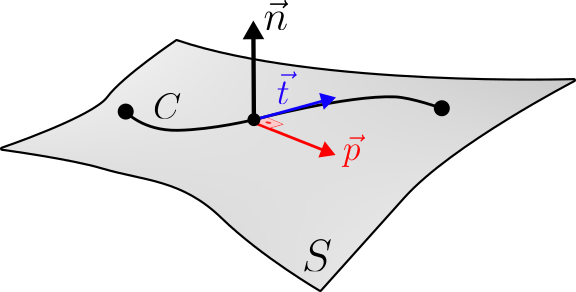
\includegraphics[scale=.4]{FOTOS/curva_geo_1.png}
    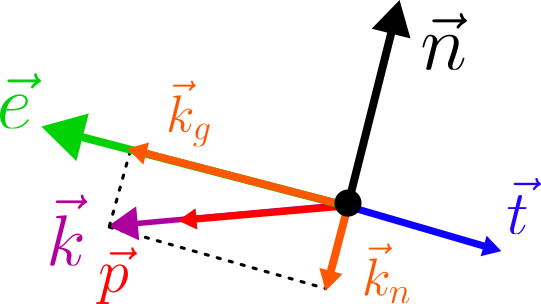
\includegraphics[scale=.4]{FOTOS/curva_geo_2.png}
\end{wrapfigure}
$$
\mathbf{k}=\mathbf{k}_n+\mathbf{k}_g
$$
donde $\mathbf{k}=k\mathbf{p}$. Si nos fijamos en el plano formado por $\mathbf{k}$ y $\mathbf{k}_n$, como $\mathbf{n}\perp \mathbf{t}\perp \mathbf{p}$, $\mathbf{k}_g\propto \mathbf{e}$, donde $\mathbf{e}=\mathbf{n}\wedge \mathbf{t}$; luego lo que ocurre es que $k_g=\mathbf{e\cdot k}=(\mathbf{n}\wedge \mathbf{t})\cdot \mathbf{k}$.\\

Si ahora usamos las fórmulas de Frenet, en parametrización natural,
\begin{gather*}
    \mathbf{k}=\Ddot{\mathbf{x}} \quad , \quad \mathbf{t}=\dot{\mathbf{x}} \quad , \quad ||\dot{\mathbf{x}}||=1 \ \forall \ s\\
    k_g=(\mathbf{n}\wedge \dot{\mathbf{x}})\cdot \ddot{\mathbf{x}}=[\ddot{\mathbf{x}}\ ,\ \dot{\mathbf{x}}\ ,\ \mathbf{n}]\\
    \boxed{k_g=\det{\mathbf{n}\ | \ \dot{\mathbf{x}}\  | \ \ddot{\mathbf{x}}}}
\end{gather*}
En parametrización arbitraria:
$$
\dv{}{S}=\dv{t}{S}\cdot \dv{}{t}=\frac{1}{||\mathbf{x}'||}\dv{}{t}
$$
luego:
\begin{gather*}
    \dot{\mathbf{x}}=\frac{\mathbf{x}'}{||\mathbf{x}'||}\longrightarrow \ddot{\mathbf{x}}=\frac{\mathbf{x}''}{||\mathbf{x}'||^2}+\frac{1}{||\mathbf{x}'||}\cancelto{\text{\parbox{2.55cm}{\small No contribuye al determinante}}}{\left ( \dv{}{t} \left ( \frac{1}{||\mathbf{x}'||} \right ) \right )}\cdot \mathbf{x}'\\
    \boxed{k_g=\frac{1}{||\mathbf{x}'||^3}\det{\mathbf{n} \ | \ \mathbf{x}' \ | \ \mathbf{x}''}}
\end{gather*}
\section{Geodésicas}
Una \emph{pregeodésica} es una es una curva con \emph{curvatura geodésica nula} en cualquier punto de la curva.\\

Una \emph{geodésica} es una curva que:
\begin{enumerate}
    \item Es \emph{pregeodésica}, $k_g=0$
    \item Tiene un vector velocidad \emph{constante}, $||\mathbf{x}'||\equiv $ const.
\end{enumerate}

Si reparametrizamos una geodésica, $k_g$ seguirá siendo nulo, pero puede que la velocidad deje de ser constante. En consecuencia, una curva pregeodésica siempre mantiene su condición de pregeodésica.\\

Por otro lado, una geodésica es una pregeodésica parametrizada en su parámetro afín, donde el parámetro afín es una transformación lineal de la longitud de arco.
$$
t_\text{afín}=aS+b\ , \qquad a,b\equiv \text{const.} 
$$
\begin{mybox}
    \underline{Ejemplo A:} $\mathbf{x}(t)=(\log t,\log t,\log t)$ es una pregeodésica
    $$
    k_g=\frac{1}{||\mathbf{x}'||}\det{\mathbf{n} \ | \ \mathbf{x}' \ | \ \mathbf{x}''}=0 \ , \ ||\mathbf{x}'||\not \equiv \text{const.}
    $$
    $
    \mathbf{x}(\Bar{t})=(\Bar{t},\Bar{t},\Bar{t}) \ (\Bar{t}=\log t)\ \iff \mathbf{x}(t)
    $ cumple que $k_g=0$ y  $||\mathbf{x}'||\equiv \text{const.}  \ \forall \ \Bar{t}$. Es decir, $\mathbf{x}(\Bar{t})$ es una geodésica.
\end{mybox}

Un resultado muy importante es que la condición de $||\mathbf{x}'||\equiv $ const. de las geodésicas implica que, en una geodésica, la aceleración es \emph{paralela a} $\mathbf{n}$. El razonamiento es el siguiente:
\begin{align*}
    \dv{}{t}||\mathbf{x}'||^2=\mathbf{0}&\implies (\mathbf{x}'\cdot \mathbf{x}')'=\mathbf{x}''\cdot \mathbf{x}' +\mathbf{x}'\cdot \mathbf{x}''=2\mathbf{x}'\cdot \mathbf{x}''=\mathbf{0}\\
    &\iff \mathbf{x}'\perp \mathbf{x}''
\end{align*}
Además, $k_g=0=(\mathbf{n}\wedge \mathbf{x}')\cdot \mathbf{x}''$. Esto significa que $\mathbf{n,x',x''}$ son coplanares, lo que implica que $\mathbf{n}\parallel \mathbf{x}''$.\\

Las consecuencias de este resultado son que las rectas (con curvatura nula) son siempre pregeodésicas en cualquier superficie que las contiene.
\begin{mybox}
    \underline{Ejemplo B:} $S$: Paraboloide hiperbólico: $\mathbf{x}(u,v)=(u,v,u^2-v^2)$.\\
    La curva $\mathbf{x}(t)=(t,t,0)$ es una recta, y por tanto una pregeodésica (además de geodésica)
\end{mybox}
\newpage
    \begin{figure}[!h]
        \centering
        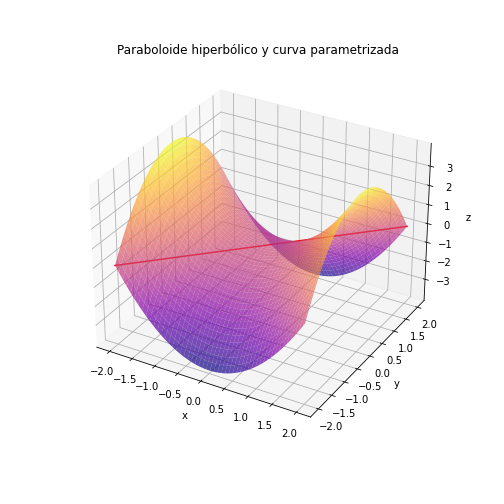
\includegraphics[scale=.5]{FOTOS/hiperb_curva.png}
        \caption*{Ejemplo B: Paraboloide hiperbólico y geodésica}
        \label{fig:ej4B}
    \end{figure}
\begin{wrapfigure}{r}{0.2\textwidth}
    \centering
    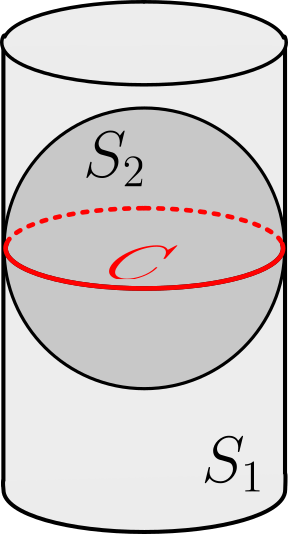
\includegraphics[scale=.35]{FOTOS/cilindro_geo.png}
\end{wrapfigure}

Si $S_1$ y $S_2$ son dos superficies tangentes entre sí a lo largo de una cierta curva $C$, entonces el hecho de que $C$ sea pregeodésica de $S_1$ implica que también lo es de $S_2$.
\subsection{Ecuación de las geodésicas}
Sea $C$ una curva sobre una superficie $S$:
$$
\mathbf{x}(s)=\mathbf{x}(u^1(s),u^2(s))=\mathbf{x}(u^\alpha (s))
$$
\begin{equation*}
    \begin{split}
        \mathbf{k}=k\mathbf{p} =\ddot{\mathbf{x}} \quad , \quad \mathbf{k}&=\mathbf{k}_g+\mathbf{k}_n\\
        &=\mathbf{k}_g+k\cdot \mathbf{n}
    \end{split}
\end{equation*}
$\mathbf{k}_g$ es la parte de $\ddot{\mathbf{x}}$ que es perpendicular a $\mathbf{n}$. 
\begin{equation*}
    \begin{split}
        \dot{\mathbf{x}}=\mathbf{x}_\alpha \cdot \dot{u}^\alpha \implies \ddot{\mathbf{x}}&=\mathbf{x}_{\alpha \beta }\cdot \dot{u}^\alpha \dot{u}^\beta +\mathbf{x}_\alpha \cdot \ddot{u}^\alpha \\
        \ref{gauss} \rightarrow &=(\Gamma _{\alpha \beta }{}^\gamma \cdot \mathbf{x}_\gamma +b_{\alpha \beta }\cdot \mathbf{n})\dot{u}^\alpha \dot{u}^\beta +\mathbf{x}_\alpha \cdot \ddot{u}^\alpha \\
        &=\underbrace{(\ddot{u}^\gamma +\Gamma _{\alpha \beta }{}^\gamma \dot{u}^\alpha \dot{u}^\beta )}_{\mathbf{k}_g}\ \mathbf{x}_\gamma + \underbrace{b_{\alpha \beta }\dot{u}^\alpha \dot{u}^\beta }_{\mathbf{k}_n}\ \mathbf{n}
    \end{split}
\end{equation*}
\WFclear
La condición de geodésica, $k_g=0$, además de que la velocidad sea constante, implica que, para este tipo de curva, se cumple la siguiente ecuación diferencial
$$
\ddot{u}^\gamma +\Gamma _{\alpha \beta }{}^\gamma \dot{u}^\alpha \dot{u}^\beta=0
$$
donde los símbolos de Christoffel se evalúan sobre la curva. Si escribimos las derivadas explícitamente, entonces:
$$
\boxed{\dv[2]{u^\gamma }{s}+\Gamma _{\alpha \beta }{}^\gamma \dv{u^\alpha }{s}\dv{u^\beta }{s}=0} \qquad \qquad \left ( \text{\small \parbox{5cm}{\begin{center}
    La estructura de esta ecuación es válida para parámetros afines $t_a=aS+b$. Al resolver esta ecuación, se obtienen las curvas en parámetro afín.
\end{center}}} \right )
$$
La ecuación es válida si trabajamos en una variedad de dimensión $n$ (en Relatividad General, se usará como parámetro $s$ el tiempo propio, $\lambda $).
\begin{mybox}
    \underline{Ejemplo C:} Plano $XY$ en coordenadas cartesianas.
    $$
    \mathbf{x}(u^1,u^2)=(u^1,u^2,0) \longrightarrow g_{\alpha \beta }=\mathbb{1}_{2\times 2} \ , \ \Gamma _{\alpha \beta }{}^\gamma =0
    $$
    Las geodésicas cumplirán:
    $$
    \dv[2]{u^\gamma }{s}=0\implies \left \{ \begin{array}{ccc}
         \dv[2]{u^1}{s}=0&\implies&u^1=as+b   \\\\
         \dv[2]{u^2}{s}=0&\implies&u^2=cs+d 
    \end{array} \right \} \ a,b,c,d \in \mathbb{R}
    $$
\end{mybox}
\section{Propiedades extremales de las geodésicas: arcos de longitud mínima}
\begin{wrapfigure}{l}{0.35\textwidth}
    \centering
    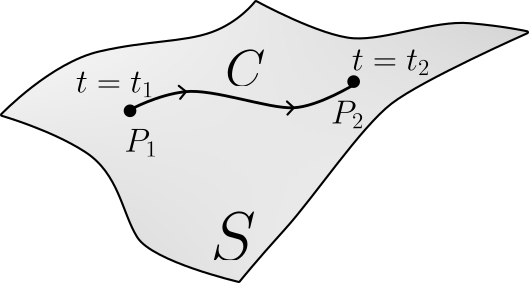
\includegraphics[scale=.4]{FOTOS/min_arco1.png}
    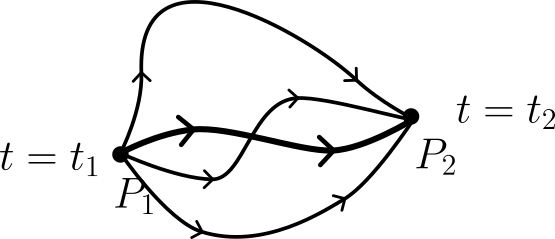
\includegraphics[scale=.35]{FOTOS/min_arco2.png}
\end{wrapfigure}
La longitud de arco de la curva $C$ contenida en la superficie $S$ que va desde el punto $P_1$ hasta el punto $P_2$ es:
$$
\ell =\int _{t_1}^{t_2} \odif{t} \sqrt{g_{\alpha \beta }(u^\alpha )'(u^\beta )'} \quad g_{\alpha \beta }=\mathbf{x}_\alpha \cdot \mathbf{x}_\beta 
$$
El integrando en la longitud de arco puede entenderse como un lagrangiano en Mecánica Clásica, que depende de las coordenadas $(u^1,u^2)$ y sus velocidades $((u^1)',(u^2)')$:
$$
\mathcal{L}(u^\alpha ,(u^\beta )')=\sqrt{g_{\alpha \beta }(u^\alpha )'(u^\beta )'}
$$
Y si pedimos que el arco que une $P_1$ y $P_2$ sea de longitud mínima, tenemos que imponer que se cumplan las \emph{ecuaciones de Euler-Lagrange} (es decir, usamos un método variacional):
$$
\boxed{\pdv{\mathcal{L}}{u^\mu }-\dv{}{t}\pdv{\mathcal{L}}{(u^\mu )'}=0}
$$
$$\hookrightarrow \pdv{\mathcal{L}}{u^\mu }=\frac{1}{2\sqrt{g_{\alpha \beta }(u^\alpha )'(u^\beta )'}}\pdv{g_{\alpha \beta }}{u^\mu }\cdot (u^\alpha )'(u^\beta )' $$
\begin{equation*}
    \begin{split}
        \hookrightarrow \pdv{\mathcal{L}}{(u^\mu )'}&=\frac{1}{2\sqrt{g_{\alpha \beta }(u^\alpha )'(u^\beta )'}}\left [ g_{\rho \sigma } \underbrace{\pdv{(u^\rho )'}{(u^\mu )'}}_{\delta ^\rho {}_\mu }\cdot (u^\sigma )'+g_{\rho \sigma }(u^\rho )'\underbrace{\pdv{(u^\sigma )'}{(u^\mu )'}}_{\delta ^\sigma {}_\rho } \right ]\\
        &=\frac{1}{\sqrt{g_{\alpha \beta }(u^\alpha )'(u^\beta )'}} g_{\mu \sigma }(u^\sigma )'
    \end{split}
\end{equation*}
Este resultado es general hasta este punto y no depende de la parametrización de $C$. A partir de ahora, realizaremos el resto del cálculo \emph{en parametrización natural}.
\begin{align*}
    \pdv{\mathcal{L}}{\dot{u}^\mu }&= g_{\mu \sigma } \dot{u}^\sigma \\
    \pdv{\mathcal{L}}{u^\mu }&=\frac{1}{2}\pdv{g_{\rho \sigma }}{u^\mu }\dot{u}^\rho \dot{u}^\sigma \\
    \dv{}{s}\left ( \pdv{\mathcal{L}}{\dot{u}^\mu } \right )&=\dot{g}_{\mu \sigma }\dot{u} ^\sigma +g_{\mu \sigma }\ddot{u}^\sigma \\
    &=\pdv{g_{\mu \sigma }}{u^\rho }\cdot \dot{u}^\rho \dot{u}^\sigma +g_{\mu \sigma }\ddot{u}^\sigma 
\end{align*}
\begin{gather*}
    g_{\mu \sigma }\ddot{u}^\sigma +\pdv{g_{\mu \sigma }}{u^\rho }-\frac{1}{2} \pdv{g_{\rho \sigma }}{u^\mu }\dot{u}^\rho \dot{u}^\sigma=0\\
    \ddot{u}^\nu +\frac{1}{2}g^{\nu \mu }\left ( \pdv{g_{\mu \sigma }}{u^\rho }+\pdv{g_{\mu \rho }}{u^\sigma }-\frac{1}{2}\pdv{g_{\rho \sigma }}{u^\mu } \right )\dot{u}^\rho \dot{u}^\sigma =0\\
    \implies \boxed{\ddot{u}^\nu +\Gamma _{\rho \sigma }{}^\nu \dot{u}^\rho \dot{u}^\sigma=0} \qquad \text{ Ecuación de las geodésicas}
\end{gather*}
Es decir, las geodésicas son arcos de longitud mínima en la superficie parametrizada S.




\clearpage


\part{Ejercicios sin corregir}

\section*{Aviso legal:}

Porque me has caído bien (Marcos o quien tenga el link de este documento), te dejo lo que tengo de ejercicios compilado en el documento. Si quieres imprimirlo avísame para que lo quite. Te aviso de que \textbf{NO} están corregidos, de hecho hay alguno que estará mal. \textbf{Úsalos a tu discreción}.\\

Enjoy $\smiley$. 





\fancyhead[L]{\emph{EJERCICIOS DEL TEMA 1}}

\chapter*{Ejercicios de tema 1}
\addcontentsline{toc}{chapter}{Tema 1}
\large
\begin{enumerate}
    \item[$\boxed{1}$] 
    \begin{enumerate}
        \item[(a)] Reconstruya la curva en $\mathbb{R}^2$ cuya curvatura es $K(S)=1/S \ (S>0)$, efectuando las integraciones en la variable $S$ con constantes de integracion nulas  y posteriormente la reparametrización $S=\exp(t-\pi/4)$.\\
        
        \item[(b)] Calcule la longitud de arco de dicha curva entre los puntos $(1/2,-1/2)$ y $(-e^\pi/2,e^\pi/2)$.
    \end{enumerate}
    \noindent\rule{\textwidth}{0.5pt}
    (a) Dada la curva paramétrica $\mathbf{x}:\mathbb{R}\longrightarrow \mathbb{R}^2$, $\mathbf{x}(S)=(x(S),y(S))$, reconstruimos la curva como sigue:
    \begin{gather*}
        \dot{\theta}(S)=K(S)\implies \theta(S)=\int K(S) \odif{S} + \cancelto{0}{\theta_0}\\
        x(S)=\int \cos(\theta(S)) \odif{S} + \cancelto{0}{x_0} \\
        y(S)=\int \sin(\theta(S)) \odif{S} + \cancelto{0}{y_0}
    \end{gather*}
    La integral de $\theta(S)$ es inmediata: $\theta(S)=\ln{S}$, ($S>0$).
    Calculamos las integrales de $x(S),y(S)$ usando el cambio de variable $x=\ln{S}$ e integrando por \textbf{partes}:
    \begin{enumerate}
        \item[$\rightarrow$] $x(S)=\int \cos(\ln{S}) \odif{S}$
        \begin{equation*}
            \begin{split}
               x(S)=I&=\int \cos(\ln{S}) \odif{S}=I=\int \cos(x)e^x \odif{x} \\
                     &=e^x\sin(x)-\int e^x \sin(x) \odif{x}\\
                     &=e^x\sin(x)+e^x\cos(x)-\underbrace{\int e^x \cos(x) \odif{x}}_{I}\\
                     &=\frac{e^x}{2}(\cos(x)+\sin(x))\\
        \implies y(S)&=\frac{S}{2}(\sin(\ln{S})+\cos(\ln{S}))
            \end{split}
        \end{equation*}
        \item[$\rightarrow$] $y(S)=\int \sin(\ln{S}) \odif{S}$
        \begin{equation*}
            \begin{split}
               y(S)=I&=\int \sin(\ln{S}) \odif{S}=\int \sin(x)e^x \odif{x} \\
                     &=-e^x\cos(x)+\int e^x \cos(x) \odif{x}\\
                     &=-e^x\cos(x)+e^x\sin(x)-\underbrace{\int e^x \sin(x) \odif{x}}_{I}\\
                     &=\frac{e^x}{2}(\cos(x)-\sin(x))\\
        \implies y(S)&=\frac{S}{2}(\sin(\ln{S})-\cos(\ln{S}))
            \end{split}
        \end{equation*}
    \end{enumerate}
        $$
        \boxed{\mathbf{x}(S)=(S/2(\sin(\ln{S})+\cos(\ln{S})),S/2(\sin(\ln{S})-\cos(\ln{S})))}
        $$

        Si reparametrizamos la curva con el parámetro $t$, obtenemos:
        $$
        \boxed{\mathbf{x}(t)=\frac{1}{\sqrt{2}}(e^{t-\pi/4}\sin(t),e^{t-\pi/4}-\cos(t))}
        $$
        que tiene esta pinta:
        \begin{figure}[!h]
            \centering
            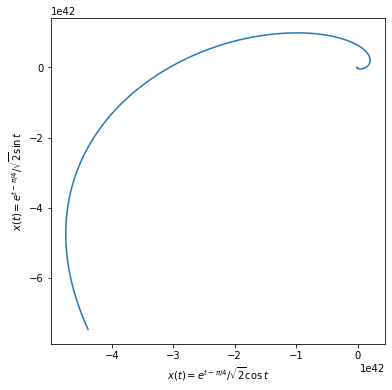
\includegraphics[scale=.5]{FOTOS/1_a.png}
            \caption*{Curva 1(a), $\mathbf{x}(t)$}
            \label{1_a}
        \end{figure}

    {\color{red} \small 10-abril-2024: Por favor, que se haga notar ese $10^{42}$ en la escala de la gráfica de la curva. El dibujo está mal (obviamente).}\\

    (b) Se puede calcular la longitud de arco en ambas parametrizaciones ya que esta es un invariante geométrico. No obstante, voy a usar la parametrización natural para aprovecharme de la propiedad de $||\dot{\mathbf{x}}(S)||=1$. La longitud de arco se calcula como:
    $$
    \ell =\int_A ^B ||\dot{\mathbf{x}}(S)|| \odif{S}=S_B-S_A
    $$

    Resolviendo el sistema de ecuaciones en cada punto, obtenemos que la $S$ debe de cumplir, en cada caso, que $\sin(\ln{S})=0$, que da soluciones periódicas de la forma $\pi k$, $k\in \mathbb{Z}$, para el logarítmo. Como estamos en $S>0$, las soluciones más próximas entre sí son $1$ y $e^\pi$, por lo que la longitud de arco es:
    $$
    \boxed{\ell=e^\pi - 1}
    $$
    \noindent\rule{\textwidth}{1pt}
    \item[$\boxed{2}$] Demuestre que la curva en $\mathbb{R}^3$ dada por $\mathbf{x}(t)=(t+ \sqrt{3}\sin t,2\cos t +2, \sqrt{3}-\sin t)$ es una hélice circular y, calculando sendos triedros de Frenet en $\mathbf{x}(0)$ y $\Tilde{\mathbf{x}}(0)$, encuentre una isometría $\Tilde{\mathbf{x}}=R\mathbf{x}+\mathbf{x}_0$ que lleve la hélice a la forma $\Tilde{\mathbf{x}}(t)=(a\cos t,a \sin t, bt)$.\\
    \noindent\rule{\textwidth}{.5pt}

    Para empezar, podemos ver que la gráfica de esta curva en $\mathbb{R}^3$ representa, efectivamente, una hélice.

    \begin{figure}[!h]
        \centering
        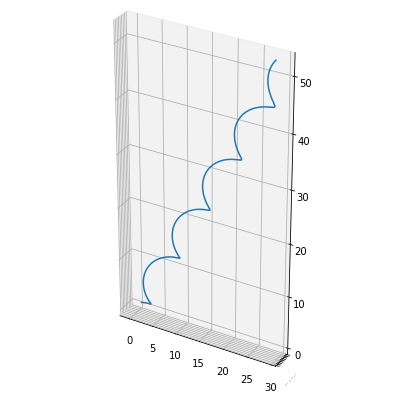
\includegraphics[scale=.5]{FOTOS/2_a.png}
        \caption*{Curva 2(a)}
        \label{fig:2a}
    \end{figure}

    Esta comienza en el punto $(0,4,0)$ y crece a lo largo de una dirección inclinada con respecto al eje vertical. En los ejemplos vistos en clase, no nos hemos encontrado en ningún momento una hélice que no tuviese como eje de simetría el eje $Z$. Por tanto, no servirá utilizar la ecuación genérica para ese tipo de hélices (que es la que proponen en el enunciado). No obstante, podremos ver que, una vez realicemos la isometría adecuada (es decir, traslaciones y rotaciones convenientes), podremos identificar la curva con la parametrización que ya conocemos. \\

    \begin{enumerate}
        \item En primer lugar, debemos demostrar que se trata de una hélice. Para ello, mostramos que la curva $\mathbf{x}(t)$ se compone de una traslación a lo largo de una dirección y de una \emph{curva plana} con radio de curvatura constante, es decir, $\rho(S)=1/K(S)\equiv$ constante. 
        \begin{equation*}
        \begin{split}
        \mathbf{x}(t)&=(t+ \sqrt{3}\sin t,2\cos t +2, \sqrt{3}-\sin t)\\
                 &=(t,2,\sqrt{3}t) \ +\ \underbrace{(\sqrt{3}\sin t,2\cos t, -\sin t)}_{\mathbf{a}(t)}
        \end{split}
        \end{equation*}

        Como habíamos enunciado, el primer término de nuestra curva es tan solo una traslación (término lineal en $t$) a lo largo de la dirección $(1,2,\sqrt{3})$. \\

        Ahora nos centramos en el siguiente término del vector. Para demostrar que se trata de una curva plana, lo más sencillo es comprobar que su \emph{vector binormal} es constante, y posteriormente calcular su radio de curvatura y ver que también es constante. \\
        Primero calculamos su primer vector del triedro de Frenet:
        $$
        \mathbf{e}_1=\frac{\mathbf{a'}(t)}{||\mathbf{a'}(t)||}=\mathbf{a'}(t)\cdot 1/2=1/2\left (\sqrt{3}\cos t,-2\sin t,-\cos t\right )
        $$
        El vector binormal $\mathbf{b}$ se obtiene como:
        $$
        \mathbf{b}(t)=\frac{\mathbf{x'}(t)\wedge \mathbf{x''}(t)}{||\mathbf{x'}(t)\wedge \mathbf{x''}(t)||}=1/4 \left ( -2,0,-2\sqrt{3} \right )\equiv \text{const.}
        $$

        Por último, la curvatura se calcula como $K=\frac{||\mathbf{x'}(t)\wedge \mathbf{x''}(t)||}{||\mathbf{x'}(t)||^3}=\frac{4}{8}=1/2$. Por tanto, el radio de curvatura es $\boxed{\rho(t)=2}$. Al tener una curva plana (vector binormal constante en la dirección de la traslación) con radio de curvatura constante, concluimos que se trata de una circunferencia y, por lo tanto, la curva parametrizada completa es una hélice.\\
        
        \textit{[Corrección]} $\mathbf{x}(t)=(t+ \sqrt{3}\sin t,2\cos t +2, \sqrt{3}-\sin t)$.\\
        
        \fbox{\parbox{4.5cm}{\textit{Hélice circular}:\\ Curva de $\mathbb{R}^3$ con sus dos curvaturas \textbf{constantes}.}} $K=\frac{w_{12}}{||\mathbf{x}'||} \ , \ \tau=\frac{w_{23}}{||\mathbf{x}'||}$
    \end{enumerate}
    \noindent\rule{\textwidth}{1pt}
    \item[$\boxed{3}$] Considere la curva $\mathbf{x}(t)=\left ( \frac{4}{5}\cos t,1-\sin t,-\frac{3}{5}\cos t \right )$. Demuestre que es una circunferencia y calcule su radio, su centro y la ecuación cartesiana del plano en que se encuentra.\\
    \noindent\rule{\textwidth}{0.5pt}
    Una circunferencia es una curva \emph{plana}, que tiene la condición de que su vector $\mathbf{b}(t)$ tiene que ser \emph{constante} para cualquier valor de $t$. Entonces, el procedimiento va a ser el siguiente:
    \begin{enumerate}
        \item Comrpobar que estamos en parametrización natural (para aliviar cálculos).
        \item Calcular $\mathbf{b}(t)$ junto con el triedro de Frenet y probar que es constante.
        \item Hallar la ecuación del plano con el vector $\mathbf{b}(t)$.
        \item Calcular su radio de curvatura y ver que es constante.
    \end{enumerate}

    En primer lugar, comprobamos que $||\mathbf{x'}(t)||=1$ (parámetro natural):
    \begin{flalign*}
        \mathbf{x'}(t)&=\left ( -\frac{4}{5}\sin t,-\cos t ,\frac{3}{5}\sin t \right ) &&\\
        ||\mathbf{x'}(t)||^2&=\frac{16}{24}\sin^2 t+\cos^2 t+\frac{9}{5}\sin^2 t=\sin^2 t+\cos^2 t\equiv 1 \smiley&&\\\\
        \implies &\text{Estamos en parametrización natural.}
    \end{flalign*}

    Ahora, calculamos los vectores del triedro de Frenet:
    \begin{flalign*}
        \dot{\mathbf{x}}(S)&=\left ( -\frac{4}{5}\sin S,-\cos S ,\frac{3}{5}\sin S \right )\equiv \mathbf{t}(S)&&\\
        \ddot{\mathbf{x}}(S)&=\left ( -\frac{4}{5}\cos S,\sin S ,\frac{3}{5}\cos S \right )&&\\\\
        \implies K(S)&=||\ddot{\mathbf{x}}(S)||=1=\rho (S) \qquad \text{(el radio de curvatura es constante)}&&\\
        \iff \mathbf{b}(S)&=\frac{\dot{\mathbf{x}}(S)\wedge \ddot{\mathbf{x}}(S)}{||\dot{\mathbf{x}}(S)\wedge \ddot{\mathbf{x}}(S)||}=\left ( -\frac{3}{5},0,-\frac{4}{5} \right )\equiv \text{const.}
    \end{flalign*}

    Es decir, que la curva es plana y su radio de curvatura es constante. Por tanto, se trata de una circunferencia. El centro de curvatura es el centro de esta circunferencia,
    $$
    \mathbf{x}_{cc}=\mathbf{x}(S)+\frac{1}{K(S)}\underbrace{\mathbf{p}(S)}_{=\mathbf{b}\wedge \mathbf{t}}=\left ( -\frac{4}{5}\cos S,\sin S ,\frac{3}{5}\cos S \right )
    $$

    La circunferencia vive en el plano \emph{perpendicular} a $\mathbf{b}(S)=\left ( -\frac{3}{5},0,-\frac{4}{5} \right )$. El plano tendrá por ecuación:
    $$
    ((x,y,z)-\overbrace{(0,0,0)}^{\in \mathbf{x}(S)})\cdot \mathbf{b}=0\implies \boxed{-3x+4z=0}
    $$

    \begin{center}
        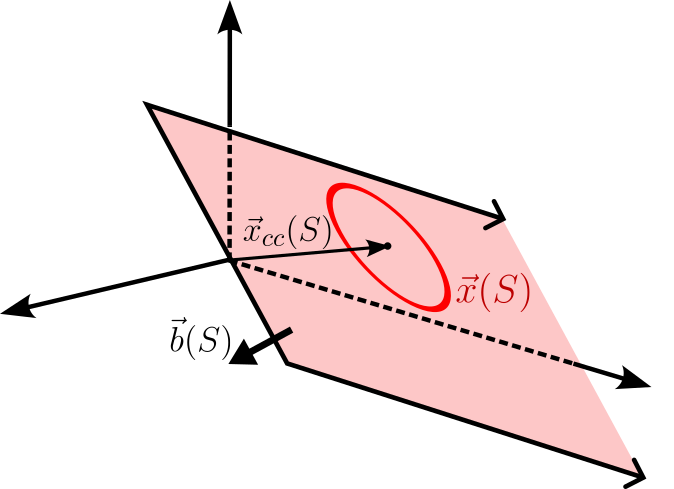
\includegraphics[scale=.5]{FOTOS/3_dibujo.png}
    \end{center}
\end{enumerate}






\fancyhead[L]{\emph{EJERCICIOS DEL TEMA 2}}

\chapter*{Ejercicios de tema 2}
\addcontentsline{toc}{chapter}{Tema 2}
\large

\begin{enumerate}
    \item[$\boxed{1}$] Sea $S$ la superficie parametrizada $\mathbf{x}(u,v)=(u\cos v,u\sin v,u^2)$, ($0<u,\ 0<v<2\pi )$, y sean $C_1$ y $C_2$ las curvas sobre $S$ dadas por $(u(t),v(t))=(t,t+1)$ y $(u(t),v(t))=(t,3-t)$, respectivamente. Calcule el ángulo que forman dichas curvas en el punto $P$ en que se cortan sobre $S$:
    \begin{enumerate}
        \item Encontrando parametrizaciones de las curvas en $\mathbb{R}^3$
        \item Operando en la base coordenada del plano $T_p(S)$ tangente a $S$ en el punto $P$.
    \end{enumerate}
\end{enumerate}
\noindent\rule{\textwidth}{0.5pt}

En primer lugar, podemos ver que la supreficie determina un paraboloide de revolución: $x(u,v)^2+y(u,v)^2=u^2=z(u,v)$. Las curvas $C_1,C_2$ dentro de este paraboloide se cortan en el punto de intersección, que cumple que:
\begin{gather*}
    C_1\cap C_2\left \{ 
    \begin{array}{cc}
        C_1:&(u,v)=(t,t+1)\\ 
        C_2:&(u,v)=(t^*,3-t^*)  
    \end{array}
    \right .\implies \begin{array}{c}
         t=t^*  \\
         1+t=3-t^* 
    \end{array}\\
    \implies t=t^*=1\iff \boxed{P(1,2)}
\end{gather*}
Las curvas tienen por ecuación:
\begin{itemize}
\item $
\mathbf{x}(\sigma_1(t))=(t\cos(1+t),t\sin(1+t),t^2)
$\\
$
\hookrightarrow \mathbf{x'}(\sigma_1(t))=(\cos(1+t)-t\sin(1+t),\sin(1+t)+t\cos(1+t),2t)
$\\
$
\hookrightarrow \mathbf{x'}(\sigma_1(1))=(\cos(2)-\sin(2),\sin(2)+\cos(2),2)
$
\item $
\mathbf{x}(\sigma_2(t))=(t\cos(3-t),t\sin(3-t),t^2)
$\\
$
\hookrightarrow \mathbf{x'}(\sigma_2(t))=(\cos(3-t)+t\sin(3-t),\sin(3-t)-t\cos(3-t),2t)
$\\
$
\hookrightarrow \mathbf{x'}(\sigma_2(1))=(\cos(2)+\sin(2),\sin(2)-\cos(2),2)
$
\end{itemize}
El coseno del ángulo formado entre las dos curvas se calcula como el del ángulo de los vectores velocidad de las curvas:
$$
\cos \theta=\frac{\mathbf{x'}(\sigma_1(1))\cdot \mathbf{x'}(\sigma_2(1))}{||\mathbf{x'}(\sigma_1(1))||\cdot ||\mathbf{x'}(\sigma_2(1))||}
$$
Calculando los módulos y el producto escalar, se llega a que:\\
$
\mathbf{x'}(\sigma_1(1))\cdot \mathbf{x'}(\sigma_2(1))=4,\ ||\mathbf{x'}(\sigma_1(1))||^2= ||\mathbf{x'}(\sigma_2(1))||^2=6
$
y finalmente:
$$
\cos \theta =\frac{4}{\sqrt{6}\sqrt{6}}=\frac{2}{3}\implies \boxed{\theta=\arccos\frac{2}{3}=48.2^\circ }
$$
\noindent\rule{\textwidth}{0.3pt}

Para calcular el ángulo con el plano $T_p(S)$, primero necesitaremos la base coordenada $\{ \mathbf{x}_\alpha  \}\equiv \{ \mathbf{x}_u,\mathbf{x}_v \}$.
$$
\mathbf{x}_u=\pdv{\mathbf{x}}{u}=(\cos v,\sin v,2u) \ , \ \mathbf{x}_v=\pdv{\mathbf{x}}{v}=(-u\sin v,u\cos v,0)
$$
En el punto $P(1,2)$, el plano tangente viene definido por $\mathbf{x}_u(1,2)=(\cos 2,\sin 2, 2)$, $\mathbf{x}_v(1,2)=(-\sin 2,\cos 2,0)$. La primera forma fundamental:
$$
g_{\mu \nu }=\left ( 
\begin{array}{cc}
     1+4u^2&0  \\
     0&u^2 
\end{array}
\right )\longrightarrow g_{\mu \nu }(1,2)=\left ( 
\begin{array}{cc}
     5&0  \\
     0&1 
\end{array} \right )
$$
El ángulo formado por dos vectores del plano $T_p(S), \mathbf{v},\mathbf{w}$, se calcula como:
$$
\cos \theta =\frac{g_{\alpha \beta }v^\alpha w^\beta }{\sqrt{g_{\mu \nu }v^\mu v^\nu }\sqrt{g_{\rho \sigma }w^\rho w^\sigma }}
$$
con las coordenadas de $\mathbf{v}$ y $\mathbf{w}$ en la base de $T_p(S)$. En esta base, estas coordenadas son: $(v^\alpha )=(1,1),\ (w^\alpha )=(1,-1)$.
$$
\cos \theta =\frac{5\cdot 1\cdot 1+1\cdot 1\cdot (-1)}{\sqrt{5\cdot 1\cdot 1+1\cdot 1\cdot 1}\sqrt{5\cdot 1\cdot 1+1\cdot (-1)\cdot (-1)}}=\frac{4}{6}=\frac{2}{3}
$$
Es decir, $\theta=48.2^\circ $.

\noindent\rule{\textwidth}{1pt}
\begin{enumerate}
    \item[$\boxed{3}$] 
    \begin{enumerate}
        \item Calcule la primera forma fundamental de la superficie parametrizada $\mathbf{x}(u^1,u^2)=(u^1+u^2,u^1-u^2,u^1u^2)$.
        \item Utilizando la regla tensorial, calcule la primera forma fundamental al efectuar la reparametrización $u^1=(\Bar{u}^1+\Bar{u}^2)/2,\ u^2=(\Bar{u}^1-\Bar{u}^2)/2$.
        \item Compruebe el resultado calculando $\mathbf{\Bar{x}}(\Bar{u}^1,\Bar{u}^2)$ y obteniendo la primera forma fundamental de esta reparametrización.
    \end{enumerate}
\end{enumerate}

\fancyhead[L]{\emph{EJERCICIOS DEL TEMA 3}}

\chapter*{Ejercicios de tema 3}
\addcontentsline{toc}{chapter}{Tema 3}
\large

\begin{enumerate}
    \item[\fbox{6}]  A partir del tensor de Riemann $R^\mu {}_{\nu \lambda \sigma }$ se definen el tensor de Ricci: $R_{\nu \sigma }=R^\mu {}_{\nu \mu \sigma }$ y la curvatura escalar $R=R^{\mu}{}_\mu $. Sabiendo que en dimensión 2 (es decir, para una superficie) el tensor de Riemann se puede escribir como: $R_{\kappa \nu \lambda \sigma }=K(g_{\kappa \lambda }g_{\nu \sigma }-g_{\kappa \sigma }g_{\nu \lambda })$, donde $K$ es la curvatura gaussiana, calcule:
    \begin{enumerate}
        \item La forma del tensor de Ricci de una superficie
        \item La curvatura escalar de una superficie
        \item $R_{\kappa \nu \lambda \sigma }\epsilon ^{\kappa \nu }\epsilon^{\lambda \sigma }$, donde $\epsilon^{\alpha \beta }$ es el tensor de Levi-Civita.
    \end{enumerate}
\end{enumerate}
\noindent\rule{\textwidth}{0.5pt}

(a) Tensor de Ricci de una superficie:
\begin{equation*}
    \begin{split}
        R_{\nu \sigma}=R^\mu {}_{\nu \mu \sigma }&=g^{\mu \kappa }R_{\kappa \nu \mu \sigma }=g^{\mu \kappa }K (g_{\kappa \lambda }g_{\nu \sigma }-g_{\kappa \sigma }g_{\nu \lambda })\\
        &=K [ g^{\mu \kappa }g_{\kappa \lambda }g_{\nu \sigma }-g^{\mu \kappa }g_{\kappa \sigma }g_{\nu \lambda } ]\\
        &=K [ \delta ^\mu {}_\mu g_{\nu \sigma }-\delta ^\mu {}_\sigma g_{\nu \lambda } ]\\
        &=K[ 2g_{\nu \sigma }-g_{\mu \sigma } ]\\
        &=\boxed{Kg_{\mu \sigma }}
    \end{split}
\end{equation*}

\end{document}
